% -----------------------------------------------------------------------------
%                                     HEADER                                    
% -----------------------------------------------------------------------------
\documentclass[a4paper, 10pt]{article}
\usepackage{jheppub}
\usepackage[T1]{fontenc}
\usepackage{colortbl,xcolor,float}
\definecolor{orange}{rgb}{1,0.5,0}
% -----------------------------------------------------------------------------
%                                   COVER PAGE                                  
% -----------------------------------------------------------------------------
\title{{
\includegraphics[scale=.4]{logo.png}}\ The LaTeX report}

\author{Generated by elijahsheridan on 23 September 2020, 11:08:18}

\abstract{
  This report has been generated automatically
  by {\sc MadAnalysis} 5.\\$~$\\ 
  Please cite:\\ 
  \begin{quote}
    \textbf{E.~Conte, B.~Fuks and G.~Serret},\\ 
    \textit{MadAnalysis 5, A User-Friendly
    Framework for Collider Phenomenology},\\ 
    Comput. Phys. Commun. {\bf 184} (2013) 222-256,\\
    arXiv:1206.1599 [hep-ph].\\ 
  \end{quote}
  To contact us:\\ 
  \begin{quote}
    \textbf{http://madanalysis.irmp.ucl.ac.be}\\
    \textbf{ma5team@iphc.cnrs.fr}\\
  \end{quote}
}

% -----------------------------------------------------------------------------
%                                 BEGIN DOCUMENT                                
% -----------------------------------------------------------------------------
\begin{document}
\maketitle
\flushbottom

% -----------------------------------------------------------------------------
%                                 SECTION Setup                                 
% -----------------------------------------------------------------------------
\newpage
\section{ Setup}

\subsection{ Command history}

\texttt{ma5>set main.currentdir = /\-Users/\-elijahsheridan/\-MG5\_aMC\_v2\_6\_5/\-axion\_pheno/\-optimization/\-ma\_scripts\\
}
\texttt{ }\texttt{ }\texttt{ma5>\# set directory where running "./\-bin/\-ma5"\\
}
\texttt{ }\texttt{ }\texttt{ma5>set main.currentdir = /\-Users/\-elijahsheridan/\-MG5\_aMC\_v2\_6\_5/\-axion\_pheno/\-madgraph\_data \# need to change this directory path --> exit and type "pwd" to get the path\\
}
\texttt{ }\texttt{ }\texttt{ma5>set main.lumi = 40\\
}
\texttt{ }\texttt{ }\texttt{ma5>set main.fom.formula = 5\\
}
\texttt{ }\texttt{ }\texttt{ma5>set main.fom.x = 0.0\\
}
\texttt{ }\texttt{ }\texttt{ma5>\# import samples --> change the path to the LHE file\\
}
\texttt{ }\texttt{ }\texttt{ma5>import /\-Users/\-elijahsheridan/\-MG5\_aMC\_v2\_6\_5/\-axion\_pheno/\-madgraph\_data/\-axion\_signal/\-axion\_signal\_gurrola\_cuts\_1MeV.lhe.gz as signal\\
}
\texttt{ }\texttt{ }\texttt{ma5>import /\-Users/\-elijahsheridan/\-MG5\_aMC\_v2\_6\_5/\-axion\_pheno/\-madgraph\_data/\-vbf\_diphoton\_background\_data/\-merged\_lhe/\-vbf\_diphoton\_background\_ht\_0\_100\_merged.lhe.gz as bg\_vbf\_0\_100\\
}
\texttt{ }\texttt{ }\texttt{ma5>import /\-Users/\-elijahsheridan/\-MG5\_aMC\_v2\_6\_5/\-axion\_pheno/\-madgraph\_data/\-vbf\_diphoton\_background\_data/\-merged\_lhe/\-vbf\_diphoton\_background\_ht\_100\_200\_merged.lhe.gz as bg\_vbf\_100\_200\\
}
\texttt{ }\texttt{ }\texttt{ma5>import /\-Users/\-elijahsheridan/\-MG5\_aMC\_v2\_6\_5/\-axion\_pheno/\-madgraph\_data/\-vbf\_diphoton\_background\_data/\-merged\_lhe/\-vbf\_diphoton\_background\_ht\_200\_400\_merged.lhe.gz as bg\_vbf\_200\_400\\
}
\texttt{ }\texttt{ }\texttt{ma5>import /\-Users/\-elijahsheridan/\-MG5\_aMC\_v2\_6\_5/\-axion\_pheno/\-madgraph\_data/\-vbf\_diphoton\_background\_data/\-merged\_lhe/\-vbf\_diphoton\_background\_ht\_400\_600\_merged.lhe.gz as bg\_vbf\_400\_600\\
}
\texttt{ }\texttt{ }\texttt{ma5>import /\-Users/\-elijahsheridan/\-MG5\_aMC\_v2\_6\_5/\-axion\_pheno/\-madgraph\_data/\-vbf\_diphoton\_background\_data/\-merged\_lhe/\-vbf\_diphoton\_background\_ht\_600\_800\_merged.lhe.gz as bg\_vbf\_600\_800\\
}
\texttt{ }\texttt{ }\texttt{ma5>import /\-Users/\-elijahsheridan/\-MG5\_aMC\_v2\_6\_5/\-axion\_pheno/\-madgraph\_data/\-vbf\_diphoton\_background\_data/\-merged\_lhe/\-vbf\_diphoton\_background\_ht\_800\_1200\_merged.lhe.gz as bg\_vbf\_800\_1200\\
}
\texttt{ }\texttt{ }\texttt{ma5>import /\-Users/\-elijahsheridan/\-MG5\_aMC\_v2\_6\_5/\-axion\_pheno/\-madgraph\_data/\-vbf\_diphoton\_background\_data/\-merged\_lhe/\-vbf\_diphoton\_background\_ht\_1200\_1600\_merged.lhe.gz as bg\_vbf\_1200\_1600\\
}
\texttt{ }\texttt{ }\texttt{ma5>import /\-Users/\-elijahsheridan/\-MG5\_aMC\_v2\_6\_5/\-axion\_pheno/\-madgraph\_data/\-vbf\_diphoton\_background\_data/\-merged\_lhe/\-vbf\_diphoton\_background\_ht\_1600\_inf\_merged.lhe.gz as bg\_vbf\_1600\_inf\\
}
\texttt{ }\texttt{ }\texttt{ma5>import /\-Users/\-elijahsheridan/\-MG5\_aMC\_v2\_6\_5/\-axion\_pheno/\-madgraph\_data/\-diphoton\_double\_isr\_background\_data/\-merged\_lhe/\-diphoton\_double\_isr\_background\_ht\_0\_100\_merged.lhe.gz as bg\_dip\_0\_100\\
}
\texttt{ }\texttt{ }\texttt{ma5>import /\-Users/\-elijahsheridan/\-MG5\_aMC\_v2\_6\_5/\-axion\_pheno/\-madgraph\_data/\-diphoton\_double\_isr\_background\_data/\-merged\_lhe/\-diphoton\_double\_isr\_background\_ht\_100\_200\_merged.lhe.gz as bg\_dip\_100\_200\\
}
\texttt{ }\texttt{ }\texttt{ma5>import /\-Users/\-elijahsheridan/\-MG5\_aMC\_v2\_6\_5/\-axion\_pheno/\-madgraph\_data/\-diphoton\_double\_isr\_background\_data/\-merged\_lhe/\-diphoton\_double\_isr\_background\_ht\_200\_400\_merged.lhe.gz as bg\_dip\_200\_400\\
}
\texttt{ }\texttt{ }\texttt{ma5>import /\-Users/\-elijahsheridan/\-MG5\_aMC\_v2\_6\_5/\-axion\_pheno/\-madgraph\_data/\-diphoton\_double\_isr\_background\_data/\-merged\_lhe/\-diphoton\_double\_isr\_background\_ht\_400\_600\_merged.lhe.gz as bg\_dip\_400\_600\\
}
\texttt{ }\texttt{ }\texttt{ma5>import /\-Users/\-elijahsheridan/\-MG5\_aMC\_v2\_6\_5/\-axion\_pheno/\-madgraph\_data/\-diphoton\_double\_isr\_background\_data/\-merged\_lhe/\-diphoton\_double\_isr\_background\_ht\_600\_800\_merged.lhe.gz as bg\_dip\_600\_800\\
}
\texttt{ }\texttt{ }\texttt{ma5>import /\-Users/\-elijahsheridan/\-MG5\_aMC\_v2\_6\_5/\-axion\_pheno/\-madgraph\_data/\-diphoton\_double\_isr\_background\_data/\-merged\_lhe/\-diphoton\_double\_isr\_background\_ht\_800\_1200\_merged.lhe.gz as bg\_dip\_800\_1200\\
}
\texttt{ }\texttt{ }\texttt{ma5>import /\-Users/\-elijahsheridan/\-MG5\_aMC\_v2\_6\_5/\-axion\_pheno/\-madgraph\_data/\-diphoton\_double\_isr\_background\_data/\-merged\_lhe/\-diphoton\_double\_isr\_background\_ht\_1200\_1600\_merged.lhe.gz as bg\_dip\_1200\_1600\\
}
\texttt{ }\texttt{ }\texttt{ma5>import /\-Users/\-elijahsheridan/\-MG5\_aMC\_v2\_6\_5/\-axion\_pheno/\-madgraph\_data/\-diphoton\_double\_isr\_background\_data/\-merged\_lhe/\-diphoton\_double\_isr\_background\_ht\_1600\_inf\_merged.lhe.gz as bg\_dip\_1600\_inf\\
}
\texttt{ }\texttt{ }\texttt{ma5>\# define bg and signal samples\\
}
\texttt{ }\texttt{ }\texttt{ma5>set signal.type = signal\\
}
\texttt{ }\texttt{ }\texttt{ma5>set bg\_vbf\_0\_100.type = background\\
}
\texttt{ }\texttt{ }\texttt{ma5>set bg\_vbf\_100\_200.type = background\\
}
\texttt{ }\texttt{ }\texttt{ma5>set bg\_vbf\_200\_400.type  = background\\
}
\texttt{ }\texttt{ }\texttt{ma5>set bg\_vbf\_400\_600.type  = background\\
}
\texttt{ }\texttt{ }\texttt{ma5>set bg\_vbf\_600\_800.type  = background\\
}
\texttt{ }\texttt{ }\texttt{ma5>set bg\_vbf\_800\_1200.type  = background\\
}
\texttt{ }\texttt{ }\texttt{ma5>set bg\_vbf\_1200\_1600.type  = background\\
}
\texttt{ }\texttt{ }\texttt{ma5>set bg\_vbf\_1600\_inf.type = background\\
}
\texttt{ }\texttt{ }\texttt{ma5>set bg\_dip\_0\_100.type = background\\
}
\texttt{ }\texttt{ }\texttt{ma5>set bg\_dip\_100\_200.type = background\\
}
\texttt{ }\texttt{ }\texttt{ma5>set bg\_dip\_200\_400.type = background\\
}
\texttt{ }\texttt{ }\texttt{ma5>set bg\_dip\_400\_600.type = background\\
}
\texttt{ }\texttt{ }\texttt{ma5>set bg\_dip\_600\_800.type = background\\
}
\texttt{ }\texttt{ }\texttt{ma5>set bg\_dip\_800\_1200.type = background\\
}
\texttt{ }\texttt{ }\texttt{ma5>set bg\_dip\_1200\_1600.type = background\\
}
\texttt{ }\texttt{ }\texttt{ma5>set bg\_dip\_1600\_inf.type = background\\
}
\texttt{ }\texttt{ }\texttt{ma5>\# a jet can be from a light quark or b quark\\
}
\texttt{ }\texttt{ }\texttt{ma5>define jets = j\\
}
\texttt{ }\texttt{ }\texttt{ma5>define e = e+ e-\\
}
\texttt{ }\texttt{ }\texttt{ma5>define mu = mu+ mu-\\
}
\texttt{ }\texttt{ }\texttt{ma5>define ta = ta+ ta-\\
}
\texttt{ }\texttt{ }\texttt{ma5>define lept = e mu ta\\
}
\texttt{ }\texttt{ }\texttt{ma5>define ax = 9000005\\
}
\texttt{ }\texttt{ }\texttt{ma5>\# cuts\\
}
\texttt{ }\texttt{ }\texttt{ma5>\# select M(a[1] a[2]) > 500\\
}
\texttt{ }\texttt{ }\texttt{ma5>\# select PT(a[1]) > 300\\
}
\texttt{ }\texttt{ }\texttt{ma5>\# select M(jets[1] jets[2]) > 750\\
}
\texttt{ }\texttt{ }\texttt{ma5>\# select sdETA(jets[1] jets[2]) > 3.6 or sdETA(jets[1] jets[2]) < -3.6\\
}
\texttt{ }\texttt{ }\texttt{ma5>select PT(jets[1]) > 30 and PT(jets[2]) > 30\\
}
\texttt{ }\texttt{ }\texttt{ma5>select sdETA(jets[1] jets[2]) > 3.6 or sdETA(jets[1] jets[2]) < -3.6\\
}
\texttt{ }\texttt{ }\texttt{ma5>select M(jets[1] jets[2]) > 750\\
}
\texttt{ }\texttt{ }\texttt{ma5>\# define which plots to make\\
}
\texttt{ }\texttt{ }\texttt{ma5>plot PT(jets[1])\\
}
\texttt{ }\texttt{ }\texttt{ma5>plot ETA(jets[1])\\
}
\texttt{ }\texttt{ }\texttt{ma5>plot PHI(jets[1])\\
}
\texttt{ }\texttt{ }\texttt{ma5>plot PT(jets[2])\\
}
\texttt{ }\texttt{ }\texttt{ma5>plot ETA(jets[2])\\
}
\texttt{ }\texttt{ }\texttt{ma5>plot PHI(jets[2])\\
}
\texttt{ }\texttt{ }\texttt{ma5>plot DELTAR(jets[1], jets[2])\\
}
\texttt{ }\texttt{ }\texttt{ma5>plot M(jets[1] jets[2])\\
}
\texttt{ }\texttt{ }\texttt{ma5>plot sdETA(jets[1] jets[2])\\
}
\texttt{ }\texttt{ }\texttt{ma5>plot M(a[1] a[2])\\
}
\texttt{ }\texttt{ }\texttt{ma5>plot PT(a[1])\\
}
\texttt{ }\texttt{ }\texttt{ma5>plot PT(a[2])\\
}
\texttt{ }\texttt{ }\texttt{ma5>plot THT\\
}
\texttt{ }\texttt{ }\texttt{ma5>plot MET\\
}
\texttt{ }\texttt{ }\texttt{ma5>plot TET\\
}
\texttt{ }\texttt{ }\texttt{ma5>plot DELTAR(a[1], a[2])\\
}
\texttt{ }\texttt{ }\texttt{ma5>plot sdETA(a[1] a[2])\\
}
\texttt{ }\texttt{ }\texttt{ma5>\#set the plot/\-graph parameters\\
}
\texttt{ }\texttt{ }\texttt{ma5>set selection[5].xmin = 0\\
}
\texttt{ }\texttt{ }\texttt{ma5>set selection[5].xmax = 2000\\
}
\texttt{ }\texttt{ }\texttt{ma5>set selection[5].nbins = 200\\
}
\texttt{ }\texttt{ }\texttt{ma5>set selection[5].rank = PTordering\\
}
\texttt{ }\texttt{ }\texttt{ma5>set selection[5].titleX = "p\_\{T\}[j\_\{1\}] (GeV)"\\
}
\texttt{ }\texttt{ }\texttt{ma5>set selection[6].xmin = -8\\
}
\texttt{ }\texttt{ }\texttt{ma5>set selection[6].xmax = 8\\
}
\texttt{ }\texttt{ }\texttt{ma5>set selection[6].nbins = 160\\
}
\texttt{ }\texttt{ }\texttt{ma5>set selection[6].rank = PTordering\\
}
\texttt{ }\texttt{ }\texttt{ma5>set selection[6].titleX = "\#eta[j\_\{1\}]"\\
}
\texttt{ }\texttt{ }\texttt{ma5>set selection[7].xmin = -3.2\\
}
\texttt{ }\texttt{ }\texttt{ma5>set selection[7].xmax = 3.2\\
}
\texttt{ }\texttt{ }\texttt{ma5>set selection[7].nbins = 64\\
}
\texttt{ }\texttt{ }\texttt{ma5>set selection[7].rank = PTordering\\
}
\texttt{ }\texttt{ }\texttt{ma5>set selection[7].titleX = "\#phi[j\_\{1\}]"\\
}
\texttt{ }\texttt{ }\texttt{ma5>set selection[8].xmin = 0\\
}
\texttt{ }\texttt{ }\texttt{ma5>set selection[8].xmax = 1000\\
}
\texttt{ }\texttt{ }\texttt{ma5>set selection[8].nbins = 100\\
}
\texttt{ }\texttt{ }\texttt{ma5>set selection[8].rank = PTordering\\
}
\texttt{ }\texttt{ }\texttt{ma5>set selection[8].titleX = "p\_\{T\}[j\_\{2\}] (GeV)"\\
}
\texttt{ }\texttt{ }\texttt{ma5>set selection[9].xmin = -8\\
}
\texttt{ }\texttt{ }\texttt{ma5>set selection[9].xmax = 8\\
}
\texttt{ }\texttt{ }\texttt{ma5>set selection[9].nbins = 160\\
}
\texttt{ }\texttt{ }\texttt{ma5>set selection[9].rank = PTordering\\
}
\texttt{ }\texttt{ }\texttt{ma5>set selection[9].titleX = "\#eta[j\_\{2\}]"\\
}
\texttt{ }\texttt{ }\texttt{ma5>set selection[10].xmin = -3.2\\
}
\texttt{ }\texttt{ }\texttt{ma5>set selection[10].xmax = 3.2\\
}
\texttt{ }\texttt{ }\texttt{ma5>set selection[10].nbins = 64\\
}
\texttt{ }\texttt{ }\texttt{ma5>set selection[10].rank = PTordering\\
}
\texttt{ }\texttt{ }\texttt{ma5>set selection[10].titleX = "\#phi[j\_\{2\}]"\\
}
\texttt{ }\texttt{ }\texttt{ma5>set selection[11].xmin = 0\\
}
\texttt{ }\texttt{ }\texttt{ma5>set selection[11].xmax = 15\\
}
\texttt{ }\texttt{ }\texttt{ma5>set selection[11].nbins = 75\\
}
\texttt{ }\texttt{ }\texttt{ma5>set selection[11].rank = PTordering\\
}
\texttt{ }\texttt{ }\texttt{ma5>set selection[11].titleX = "\#DeltaR[j\_\{1\},j\_\{2\}]"\\
}
\texttt{ }\texttt{ }\texttt{ma5>set selection[12].xmin = 120\\
}
\texttt{ }\texttt{ }\texttt{ma5>set selection[12].xmax = 2000\\
}
\texttt{ }\texttt{ }\texttt{ma5>set selection[12].nbins = 160\\
}
\texttt{ }\texttt{ }\texttt{ma5>set selection[12].rank = PTordering\\
}
\texttt{ }\texttt{ }\texttt{ma5>set selection[12].titleX = "M[j\_\{1\},j\_\{2\}] (GeV)"\\
}
\texttt{ }\texttt{ }\texttt{ma5>set selection[13].xmin = 2.4\\
}
\texttt{ }\texttt{ }\texttt{ma5>set selection[13].xmax = 8\\
}
\texttt{ }\texttt{ }\texttt{ma5>set selection[13].titleX = "\#Delta\#eta(j\_\{1\},j\_\{2\})"\\
}
\texttt{ }\texttt{ }\texttt{ma5>set selection[14].xmin = 0\\
}
\texttt{ }\texttt{ }\texttt{ma5>set selection[14].xmax = 1000\\
}
\texttt{ }\texttt{ }\texttt{ma5>set selection[14].nbins = 400\\
}
\texttt{ }\texttt{ }\texttt{ma5>set selection[14].rank = PTordering\\
}
\texttt{ }\texttt{ }\texttt{ma5>set selection[14].titleX = "M[a\_\{1\},a\_\{2\}] (GeV)"\\
}
\texttt{ }\texttt{ }\texttt{ma5>set selection[15].xmin = 0\\
}
\texttt{ }\texttt{ }\texttt{ma5>set selection[15].xmax = 1000\\
}
\texttt{ }\texttt{ }\texttt{ma5>set selection[15].nbins = 80\\
}
\texttt{ }\texttt{ }\texttt{ma5>set selection[15].rank = PTordering\\
}
\texttt{ }\texttt{ }\texttt{ma5>set selection[15].titleX = "p\_\{T\}[a\_\{1\}]"\\
}
\texttt{ }\texttt{ }\texttt{ma5>set selection[16].xmin = 0\\
}
\texttt{ }\texttt{ }\texttt{ma5>set selection[16].xmax = 2000\\
}
\texttt{ }\texttt{ }\texttt{ma5>set selection[16].nbins = 400\\
}
\texttt{ }\texttt{ }\texttt{ma5>set selection[16].rank = PTordering\\
}
\texttt{ }\texttt{ }\texttt{ma5>set selection[16].titleX = "p\_\{T\}[a\_\{2\}] (GeV)"\\
}
\texttt{ }\texttt{ }\texttt{ma5>set selection[17].xmin = 0\\
}
\texttt{ }\texttt{ }\texttt{ma5>set selection[17].xmax = 4000\\
}
\texttt{ }\texttt{ }\texttt{ma5>set selection[17].nbins = 80\\
}
\texttt{ }\texttt{ }\texttt{ma5>set selection[17].rank = PTordering\\
}
\texttt{ }\texttt{ }\texttt{ma5>set selection[17].titleX = "THT"\\
}
\texttt{ }\texttt{ }\texttt{ma5>set selection[18].xmin = 0\\
}
\texttt{ }\texttt{ }\texttt{ma5>set selection[18].xmax = 1000\\
}
\texttt{ }\texttt{ }\texttt{ma5>set selection[18].nbins = 200\\
}
\texttt{ }\texttt{ }\texttt{ma5>set selection[18].rank = PTordering\\
}
\texttt{ }\texttt{ }\texttt{ma5>set selection[18].titleX = "MET"\\
}
\texttt{ }\texttt{ }\texttt{ma5>set selection[19].xmin = 0\\
}
\texttt{ }\texttt{ }\texttt{ma5>set selection[19].xmax = 8000\\
}
\texttt{ }\texttt{ }\texttt{ma5>set selection[19].nbins = 80\\
}
\texttt{ }\texttt{ }\texttt{ma5>set selection[19].rank = PTordering\\
}
\texttt{ }\texttt{ }\texttt{ma5>set selection[19].titleX = "TET"\\
}
\texttt{ }\texttt{ }\texttt{ma5>submit vbf\_eff\_flow\_chart\\
}
\texttt{ }\texttt{ }\subsection{ Configuration}

\begin{itemize}
  \item MadAnalysis version 1.6.33 (2017/\-11/\-20).
   \item Histograms given for an integrated luminosity of \textcolor{blue}{40.0}\textcolor{blue}{ fb}$^{\textcolor{blue}{-1}}$\textcolor{blue}{.}
\textcolor{blue}{}
\end{itemize}
% -----------------------------------------------------------------------------
%                                SECTION Datasets                               
% -----------------------------------------------------------------------------
\newpage
\section{ Datasets}

\subsection{ signal}

\begin{itemize}
  \item Samples stored in the directory: \textcolor{blue}{/\-Users/\-elijahsheridan/\-MG5\_aMC\_v2\_6\_5/\-axion\_pheno/\-post\_optimization\_studies/\-mad\_analyses} .
   \item Sample consisting of: \textcolor{blue}{signal}  events.
   \item Generated events: \textcolor{blue}{1000000 }  events.
   \item Normalization to the luminosity: \textcolor{blue}{4094}\textcolor{blue}{ +/\-- }\textcolor{blue}{2 }  events.
   \item Ratio (event weight): \textcolor{blue}{0.0041 } .  
 
\end{itemize}
\begin{table}[H]
  \begin{center}
    \begin{tabular}{|m{55.0mm}|m{25.0mm}|m{30.0mm}|m{30.0mm}|}
      \hline
      {\cellcolor{yellow}         Path to the event file}& {\cellcolor{yellow}         Nr. of events}& {\cellcolor{yellow}         Cross section (pb)}& {\cellcolor{yellow}         Negative wgts (\%)}\\
      \hline
      {\cellcolor{white}          /\-Users/\-elijahsheridan/\-MG5\_aMC\_v2\_6\_5/\-axion\_pheno/\-madgraph\_data/\-axion\_signal/\-axion\_signal\_gurrola\_cuts\_1MeV.lhe.gz}& {\cellcolor{white}          1000000}& {\cellcolor{white}          0.102 @ 0.028\%}& {\cellcolor{white}          0.0}\\
\hline
    \end{tabular}
  \end{center}
\end{table}

\subsection{ bg\_vbf\_0\_100}

\begin{itemize}
  \item Samples stored in the directory: \textcolor{blue}{/\-Users/\-elijahsheridan/\-MG5\_aMC\_v2\_6\_5/\-axion\_pheno/\-post\_optimization\_studies/\-mad\_analyses} .
   \item Sample consisting of: \textcolor{blue}{background}  events.
   \item Generated events: \textcolor{blue}{1000000 }  events.
   \item Normalization to the luminosity: \textcolor{blue}{12150}\textcolor{blue}{ +/\-- }\textcolor{blue}{24 }  events.
   \item Ratio (event weight): \textcolor{blue}{0.012 } .  
 
\end{itemize}
\begin{table}[H]
  \begin{center}
    \begin{tabular}{|m{55.0mm}|m{25.0mm}|m{30.0mm}|m{30.0mm}|}
      \hline
      {\cellcolor{yellow}         Path to the event file}& {\cellcolor{yellow}         Nr. of events}& {\cellcolor{yellow}         Cross section (pb)}& {\cellcolor{yellow}         Negative wgts (\%)}\\
      \hline
      {\cellcolor{white}          /\-Users/\-elijahsheridan/\-MG5\_aMC\_v2\_6\_5/\-axion\_pheno/\-madgraph\_data/\-vbf\_diphoton\_background\_data/\-merged\_lhe/\-vbf\_diphoton\_background\_ht\_0\_100\_merged.lhe.gz}& {\cellcolor{white}          1000000}& {\cellcolor{white}          0.304 @ 0.19\%}& {\cellcolor{white}          0.0}\\
\hline
    \end{tabular}
  \end{center}
\end{table}

\subsection{ bg\_vbf\_100\_200}

\begin{itemize}
  \item Samples stored in the directory: \textcolor{blue}{/\-Users/\-elijahsheridan/\-MG5\_aMC\_v2\_6\_5/\-axion\_pheno/\-post\_optimization\_studies/\-mad\_analyses} .
   \item Sample consisting of: \textcolor{blue}{background}  events.
   \item Generated events: \textcolor{blue}{965662 }  events.
   \item Normalization to the luminosity: \textcolor{blue}{9695}\textcolor{blue}{ +/\-- }\textcolor{blue}{17 }  events.
   \item Ratio (event weight): \textcolor{blue}{0.01 } .  
 
\end{itemize}
\begin{table}[H]
  \begin{center}
    \begin{tabular}{|m{55.0mm}|m{25.0mm}|m{30.0mm}|m{30.0mm}|}
      \hline
      {\cellcolor{yellow}         Path to the event file}& {\cellcolor{yellow}         Nr. of events}& {\cellcolor{yellow}         Cross section (pb)}& {\cellcolor{yellow}         Negative wgts (\%)}\\
      \hline
      {\cellcolor{white}          /\-Users/\-elijahsheridan/\-MG5\_aMC\_v2\_6\_5/\-axion\_pheno/\-madgraph\_data/\-vbf\_diphoton\_background\_data/\-merged\_lhe/\-vbf\_diphoton\_background\_ht\_100\_200\_merged.lhe.gz}& {\cellcolor{white}          965662}& {\cellcolor{white}          0.242 @ 0.17\%}& {\cellcolor{white}          0.0}\\
\hline
    \end{tabular}
  \end{center}
\end{table}

\subsection{ bg\_vbf\_200\_400}

\begin{itemize}
  \item Samples stored in the directory: \textcolor{blue}{/\-Users/\-elijahsheridan/\-MG5\_aMC\_v2\_6\_5/\-axion\_pheno/\-post\_optimization\_studies/\-mad\_analyses} .
   \item Sample consisting of: \textcolor{blue}{background}  events.
   \item Generated events: \textcolor{blue}{984165 }  events.
   \item Normalization to the luminosity: \textcolor{blue}{5413}\textcolor{blue}{ +/\-- }\textcolor{blue}{11 }  events.
   \item Ratio (event weight): \textcolor{blue}{0.0055 } .  
 
\end{itemize}
\begin{table}[H]
  \begin{center}
    \begin{tabular}{|m{55.0mm}|m{25.0mm}|m{30.0mm}|m{30.0mm}|}
      \hline
      {\cellcolor{yellow}         Path to the event file}& {\cellcolor{yellow}         Nr. of events}& {\cellcolor{yellow}         Cross section (pb)}& {\cellcolor{yellow}         Negative wgts (\%)}\\
      \hline
      {\cellcolor{white}          /\-Users/\-elijahsheridan/\-MG5\_aMC\_v2\_6\_5/\-axion\_pheno/\-madgraph\_data/\-vbf\_diphoton\_background\_data/\-merged\_lhe/\-vbf\_diphoton\_background\_ht\_200\_400\_merged.lhe.gz}& {\cellcolor{white}          984165}& {\cellcolor{white}          0.135 @ 0.2\%}& {\cellcolor{white}          0.0}\\
\hline
    \end{tabular}
  \end{center}
\end{table}

\subsection{ bg\_vbf\_400\_600}

\begin{itemize}
  \item Samples stored in the directory: \textcolor{blue}{/\-Users/\-elijahsheridan/\-MG5\_aMC\_v2\_6\_5/\-axion\_pheno/\-post\_optimization\_studies/\-mad\_analyses} .
   \item Sample consisting of: \textcolor{blue}{background}  events.
   \item Generated events: \textcolor{blue}{1000000 }  events.
   \item Normalization to the luminosity: \textcolor{blue}{986}\textcolor{blue}{ +/\-- }\textcolor{blue}{2 }  events.
   \item Ratio (event weight): \textcolor{blue}{0.00099 } .  
 
\end{itemize}
\begin{table}[H]
  \begin{center}
    \begin{tabular}{|m{55.0mm}|m{25.0mm}|m{30.0mm}|m{30.0mm}|}
      \hline
      {\cellcolor{yellow}         Path to the event file}& {\cellcolor{yellow}         Nr. of events}& {\cellcolor{yellow}         Cross section (pb)}& {\cellcolor{yellow}         Negative wgts (\%)}\\
      \hline
      {\cellcolor{white}          /\-Users/\-elijahsheridan/\-MG5\_aMC\_v2\_6\_5/\-axion\_pheno/\-madgraph\_data/\-vbf\_diphoton\_background\_data/\-merged\_lhe/\-vbf\_diphoton\_background\_ht\_400\_600\_merged.lhe.gz}& {\cellcolor{white}          1000000}& {\cellcolor{white}          0.0247 @ 0.14\%}& {\cellcolor{white}          0.0}\\
\hline
    \end{tabular}
  \end{center}
\end{table}

\subsection{ bg\_vbf\_600\_800}

\begin{itemize}
  \item Samples stored in the directory: \textcolor{blue}{/\-Users/\-elijahsheridan/\-MG5\_aMC\_v2\_6\_5/\-axion\_pheno/\-post\_optimization\_studies/\-mad\_analyses} .
   \item Sample consisting of: \textcolor{blue}{background}  events.
   \item Generated events: \textcolor{blue}{1000000 }  events.
   \item Normalization to the luminosity: \textcolor{blue}{252}\textcolor{blue}{ +/\-- }\textcolor{blue}{1 }  events.
   \item Ratio (event weight): \textcolor{blue}{0.00025 } .  
 
\end{itemize}
\begin{table}[H]
  \begin{center}
    \begin{tabular}{|m{55.0mm}|m{25.0mm}|m{30.0mm}|m{30.0mm}|}
      \hline
      {\cellcolor{yellow}         Path to the event file}& {\cellcolor{yellow}         Nr. of events}& {\cellcolor{yellow}         Cross section (pb)}& {\cellcolor{yellow}         Negative wgts (\%)}\\
      \hline
      {\cellcolor{white}          /\-Users/\-elijahsheridan/\-MG5\_aMC\_v2\_6\_5/\-axion\_pheno/\-madgraph\_data/\-vbf\_diphoton\_background\_data/\-merged\_lhe/\-vbf\_diphoton\_background\_ht\_600\_800\_merged.lhe.gz}& {\cellcolor{white}          1000000}& {\cellcolor{white}          0.0063 @ 0.13\%}& {\cellcolor{white}          0.0}\\
\hline
    \end{tabular}
  \end{center}
\end{table}

\subsection{ bg\_vbf\_800\_1200}

\begin{itemize}
  \item Samples stored in the directory: \textcolor{blue}{/\-Users/\-elijahsheridan/\-MG5\_aMC\_v2\_6\_5/\-axion\_pheno/\-post\_optimization\_studies/\-mad\_analyses} .
   \item Sample consisting of: \textcolor{blue}{background}  events.
   \item Generated events: \textcolor{blue}{400839 }  events.
   \item Normalization to the luminosity: \textcolor{blue}{114}\textcolor{blue}{ +/\-- }\textcolor{blue}{1 }  events.
   \item Ratio (event weight): \textcolor{blue}{0.00028 } .  
 
\end{itemize}
\begin{table}[H]
  \begin{center}
    \begin{tabular}{|m{55.0mm}|m{25.0mm}|m{30.0mm}|m{30.0mm}|}
      \hline
      {\cellcolor{yellow}         Path to the event file}& {\cellcolor{yellow}         Nr. of events}& {\cellcolor{yellow}         Cross section (pb)}& {\cellcolor{yellow}         Negative wgts (\%)}\\
      \hline
      {\cellcolor{white}          /\-Users/\-elijahsheridan/\-MG5\_aMC\_v2\_6\_5/\-axion\_pheno/\-madgraph\_data/\-vbf\_diphoton\_background\_data/\-merged\_lhe/\-vbf\_diphoton\_background\_ht\_800\_1200\_merged.lhe.gz}& {\cellcolor{white}          400839}& {\cellcolor{white}          0.00287 @ 0.16\%}& {\cellcolor{white}          0.0}\\
\hline
    \end{tabular}
  \end{center}
\end{table}

\subsection{ bg\_vbf\_1200\_1600}

\begin{itemize}
  \item Samples stored in the directory: \textcolor{blue}{/\-Users/\-elijahsheridan/\-MG5\_aMC\_v2\_6\_5/\-axion\_pheno/\-post\_optimization\_studies/\-mad\_analyses} .
   \item Sample consisting of: \textcolor{blue}{background}  events.
   \item Generated events: \textcolor{blue}{953803 }  events.
   \item Normalization to the luminosity: \textcolor{blue}{20}\textcolor{blue}{ +/\-- }\textcolor{blue}{1 }  events.
   \item Ratio (event weight): \textcolor{blue}{2.1e-05 } .  
 
\end{itemize}
\begin{table}[H]
  \begin{center}
    \begin{tabular}{|m{55.0mm}|m{25.0mm}|m{30.0mm}|m{30.0mm}|}
      \hline
      {\cellcolor{yellow}         Path to the event file}& {\cellcolor{yellow}         Nr. of events}& {\cellcolor{yellow}         Cross section (pb)}& {\cellcolor{yellow}         Negative wgts (\%)}\\
      \hline
      {\cellcolor{white}          /\-Users/\-elijahsheridan/\-MG5\_aMC\_v2\_6\_5/\-axion\_pheno/\-madgraph\_data/\-vbf\_diphoton\_background\_data/\-merged\_lhe/\-vbf\_diphoton\_background\_ht\_1200\_1600\_merged.lhe.gz}& {\cellcolor{white}          953803}& {\cellcolor{white}          0.000515 @ 0.16\%}& {\cellcolor{white}          0.0}\\
\hline
    \end{tabular}
  \end{center}
\end{table}

\subsection{ bg\_vbf\_1600\_inf}

\begin{itemize}
  \item Samples stored in the directory: \textcolor{blue}{/\-Users/\-elijahsheridan/\-MG5\_aMC\_v2\_6\_5/\-axion\_pheno/\-post\_optimization\_studies/\-mad\_analyses} .
   \item Sample consisting of: \textcolor{blue}{background}  events.
   \item Generated events: \textcolor{blue}{270148 }  events.
   \item Normalization to the luminosity: \textcolor{blue}{7}\textcolor{blue}{ +/\-- }\textcolor{blue}{1 }  events.
   \item Ratio (event weight): \textcolor{blue}{2.6e-05 } .  
 
\end{itemize}
\begin{table}[H]
  \begin{center}
    \begin{tabular}{|m{55.0mm}|m{25.0mm}|m{30.0mm}|m{30.0mm}|}
      \hline
      {\cellcolor{yellow}         Path to the event file}& {\cellcolor{yellow}         Nr. of events}& {\cellcolor{yellow}         Cross section (pb)}& {\cellcolor{yellow}         Negative wgts (\%)}\\
      \hline
      {\cellcolor{white}          /\-Users/\-elijahsheridan/\-MG5\_aMC\_v2\_6\_5/\-axion\_pheno/\-madgraph\_data/\-vbf\_diphoton\_background\_data/\-merged\_lhe/\-vbf\_diphoton\_background\_ht\_1600\_inf\_merged.lhe.gz}& {\cellcolor{white}          270148}& {\cellcolor{white}          0.000191 @ 0.11\%}& {\cellcolor{white}          0.0}\\
\hline
    \end{tabular}
  \end{center}
\end{table}

\subsection{ bg\_dip\_0\_100}

\begin{itemize}
  \item Samples stored in the directory: \textcolor{blue}{/\-Users/\-elijahsheridan/\-MG5\_aMC\_v2\_6\_5/\-axion\_pheno/\-post\_optimization\_studies/\-mad\_analyses} .
   \item Sample consisting of: \textcolor{blue}{background}  events.
   \item Generated events: \textcolor{blue}{1040000 }  events.
   \item Normalization to the luminosity: \textcolor{blue}{2710847}\textcolor{blue}{ +/\-- }\textcolor{blue}{4614 }  events.
   \item\textcolor{red}{Ratio (event weight): }\textcolor{red}{2.6 }\textcolor{red}{ - warning: please generate more events (weight larger than 1)!}
\textcolor{red}{}
\end{itemize}
\begin{table}[H]
  \begin{center}
    \begin{tabular}{|m{55.0mm}|m{25.0mm}|m{30.0mm}|m{30.0mm}|}
      \hline
      {\cellcolor{yellow}         Path to the event file}& {\cellcolor{yellow}         Nr. of events}& {\cellcolor{yellow}         Cross section (pb)}& {\cellcolor{yellow}         Negative wgts (\%)}\\
      \hline
      {\cellcolor{white}          /\-Users/\-elijahsheridan/\-MG5\_aMC\_v2\_6\_5/\-axion\_pheno/\-madgraph\_data/\-diphoton\_double\_isr\_background\_data/\-merged\_lhe/\-diphoton\_double\_isr\_background\_ht\_0\_100\_merged.lhe.gz}& {\cellcolor{white}          1040000}& {\cellcolor{white}          67.8 @ 0.17\%}& {\cellcolor{white}          0.0}\\
\hline
    \end{tabular}
  \end{center}
\end{table}

\subsection{ bg\_dip\_100\_200}

\begin{itemize}
  \item Samples stored in the directory: \textcolor{blue}{/\-Users/\-elijahsheridan/\-MG5\_aMC\_v2\_6\_5/\-axion\_pheno/\-post\_optimization\_studies/\-mad\_analyses} .
   \item Sample consisting of: \textcolor{blue}{background}  events.
   \item Generated events: \textcolor{blue}{1040000 }  events.
   \item Normalization to the luminosity: \textcolor{blue}{1095362}\textcolor{blue}{ +/\-- }\textcolor{blue}{1528 }  events.
   \item\textcolor{red}{Ratio (event weight): }\textcolor{red}{1.1 }\textcolor{red}{ - warning: please generate more events (weight larger than 1)!}
\textcolor{red}{}
\end{itemize}
\begin{table}[H]
  \begin{center}
    \begin{tabular}{|m{55.0mm}|m{25.0mm}|m{30.0mm}|m{30.0mm}|}
      \hline
      {\cellcolor{yellow}         Path to the event file}& {\cellcolor{yellow}         Nr. of events}& {\cellcolor{yellow}         Cross section (pb)}& {\cellcolor{yellow}         Negative wgts (\%)}\\
      \hline
      {\cellcolor{white}          /\-Users/\-elijahsheridan/\-MG5\_aMC\_v2\_6\_5/\-axion\_pheno/\-madgraph\_data/\-diphoton\_double\_isr\_background\_data/\-merged\_lhe/\-diphoton\_double\_isr\_background\_ht\_100\_200\_merged.lhe.gz}& {\cellcolor{white}          1040000}& {\cellcolor{white}          27.4 @ 0.14\%}& {\cellcolor{white}          0.0}\\
\hline
    \end{tabular}
  \end{center}
\end{table}

\subsection{ bg\_dip\_200\_400}

\begin{itemize}
  \item Samples stored in the directory: \textcolor{blue}{/\-Users/\-elijahsheridan/\-MG5\_aMC\_v2\_6\_5/\-axion\_pheno/\-post\_optimization\_studies/\-mad\_analyses} .
   \item Sample consisting of: \textcolor{blue}{background}  events.
   \item Generated events: \textcolor{blue}{1040000 }  events.
   \item Normalization to the luminosity: \textcolor{blue}{239548}\textcolor{blue}{ +/\-- }\textcolor{blue}{414 }  events.
   \item Ratio (event weight): \textcolor{blue}{0.23 } .  
 
\end{itemize}
\begin{table}[H]
  \begin{center}
    \begin{tabular}{|m{55.0mm}|m{25.0mm}|m{30.0mm}|m{30.0mm}|}
      \hline
      {\cellcolor{yellow}         Path to the event file}& {\cellcolor{yellow}         Nr. of events}& {\cellcolor{yellow}         Cross section (pb)}& {\cellcolor{yellow}         Negative wgts (\%)}\\
      \hline
      {\cellcolor{white}          /\-Users/\-elijahsheridan/\-MG5\_aMC\_v2\_6\_5/\-axion\_pheno/\-madgraph\_data/\-diphoton\_double\_isr\_background\_data/\-merged\_lhe/\-diphoton\_double\_isr\_background\_ht\_200\_400\_merged.lhe.gz}& {\cellcolor{white}          1040000}& {\cellcolor{white}          5.99 @ 0.17\%}& {\cellcolor{white}          0.0}\\
\hline
    \end{tabular}
  \end{center}
\end{table}

\subsection{ bg\_dip\_400\_600}

\begin{itemize}
  \item Samples stored in the directory: \textcolor{blue}{/\-Users/\-elijahsheridan/\-MG5\_aMC\_v2\_6\_5/\-axion\_pheno/\-post\_optimization\_studies/\-mad\_analyses} .
   \item Sample consisting of: \textcolor{blue}{background}  events.
   \item Generated events: \textcolor{blue}{1040000 }  events.
   \item Normalization to the luminosity: \textcolor{blue}{28798}\textcolor{blue}{ +/\-- }\textcolor{blue}{53 }  events.
   \item Ratio (event weight): \textcolor{blue}{0.028 } .  
 
\end{itemize}
\begin{table}[H]
  \begin{center}
    \begin{tabular}{|m{55.0mm}|m{25.0mm}|m{30.0mm}|m{30.0mm}|}
      \hline
      {\cellcolor{yellow}         Path to the event file}& {\cellcolor{yellow}         Nr. of events}& {\cellcolor{yellow}         Cross section (pb)}& {\cellcolor{yellow}         Negative wgts (\%)}\\
      \hline
      {\cellcolor{white}          /\-Users/\-elijahsheridan/\-MG5\_aMC\_v2\_6\_5/\-axion\_pheno/\-madgraph\_data/\-diphoton\_double\_isr\_background\_data/\-merged\_lhe/\-diphoton\_double\_isr\_background\_ht\_400\_600\_merged.lhe.gz}& {\cellcolor{white}          1040000}& {\cellcolor{white}          0.72 @ 0.18\%}& {\cellcolor{white}          0.0}\\
\hline
    \end{tabular}
  \end{center}
\end{table}

\subsection{ bg\_dip\_600\_800}

\begin{itemize}
  \item Samples stored in the directory: \textcolor{blue}{/\-Users/\-elijahsheridan/\-MG5\_aMC\_v2\_6\_5/\-axion\_pheno/\-post\_optimization\_studies/\-mad\_analyses} .
   \item Sample consisting of: \textcolor{blue}{background}  events.
   \item Generated events: \textcolor{blue}{662009 }  events.
   \item Normalization to the luminosity: \textcolor{blue}{6674}\textcolor{blue}{ +/\-- }\textcolor{blue}{28 }  events.
   \item Ratio (event weight): \textcolor{blue}{0.01 } .  
 
\end{itemize}
\begin{table}[H]
  \begin{center}
    \begin{tabular}{|m{55.0mm}|m{25.0mm}|m{30.0mm}|m{30.0mm}|}
      \hline
      {\cellcolor{yellow}         Path to the event file}& {\cellcolor{yellow}         Nr. of events}& {\cellcolor{yellow}         Cross section (pb)}& {\cellcolor{yellow}         Negative wgts (\%)}\\
      \hline
      {\cellcolor{white}          /\-Users/\-elijahsheridan/\-MG5\_aMC\_v2\_6\_5/\-axion\_pheno/\-madgraph\_data/\-diphoton\_double\_isr\_background\_data/\-merged\_lhe/\-diphoton\_double\_isr\_background\_ht\_600\_800\_merged.lhe.gz}& {\cellcolor{white}          662009}& {\cellcolor{white}          0.167 @ 0.41\%}& {\cellcolor{white}          0.0}\\
\hline
    \end{tabular}
  \end{center}
\end{table}

\subsection{ bg\_dip\_800\_1200}

\begin{itemize}
  \item Samples stored in the directory: \textcolor{blue}{/\-Users/\-elijahsheridan/\-MG5\_aMC\_v2\_6\_5/\-axion\_pheno/\-post\_optimization\_studies/\-mad\_analyses} .
   \item Sample consisting of: \textcolor{blue}{background}  events.
   \item Generated events: \textcolor{blue}{1040000 }  events.
   \item Normalization to the luminosity: \textcolor{blue}{2942}\textcolor{blue}{ +/\-- }\textcolor{blue}{6 }  events.
   \item Ratio (event weight): \textcolor{blue}{0.0028 } .  
 
\end{itemize}
\begin{table}[H]
  \begin{center}
    \begin{tabular}{|m{55.0mm}|m{25.0mm}|m{30.0mm}|m{30.0mm}|}
      \hline
      {\cellcolor{yellow}         Path to the event file}& {\cellcolor{yellow}         Nr. of events}& {\cellcolor{yellow}         Cross section (pb)}& {\cellcolor{yellow}         Negative wgts (\%)}\\
      \hline
      {\cellcolor{white}          /\-Users/\-elijahsheridan/\-MG5\_aMC\_v2\_6\_5/\-axion\_pheno/\-madgraph\_data/\-diphoton\_double\_isr\_background\_data/\-merged\_lhe/\-diphoton\_double\_isr\_background\_ht\_800\_1200\_merged.lhe.gz}& {\cellcolor{white}          1040000}& {\cellcolor{white}          0.0736 @ 0.17\%}& {\cellcolor{white}          0.0}\\
\hline
    \end{tabular}
  \end{center}
\end{table}

\subsection{ bg\_dip\_1200\_1600}

\begin{itemize}
  \item Samples stored in the directory: \textcolor{blue}{/\-Users/\-elijahsheridan/\-MG5\_aMC\_v2\_6\_5/\-axion\_pheno/\-post\_optimization\_studies/\-mad\_analyses} .
   \item Sample consisting of: \textcolor{blue}{background}  events.
   \item Generated events: \textcolor{blue}{337115 }  events.
   \item Normalization to the luminosity: \textcolor{blue}{513}\textcolor{blue}{ +/\-- }\textcolor{blue}{3 }  events.
   \item Ratio (event weight): \textcolor{blue}{0.0015 } .  
 
\end{itemize}
\begin{table}[H]
  \begin{center}
    \begin{tabular}{|m{55.0mm}|m{25.0mm}|m{30.0mm}|m{30.0mm}|}
      \hline
      {\cellcolor{yellow}         Path to the event file}& {\cellcolor{yellow}         Nr. of events}& {\cellcolor{yellow}         Cross section (pb)}& {\cellcolor{yellow}         Negative wgts (\%)}\\
      \hline
      {\cellcolor{white}          /\-Users/\-elijahsheridan/\-MG5\_aMC\_v2\_6\_5/\-axion\_pheno/\-madgraph\_data/\-diphoton\_double\_isr\_background\_data/\-merged\_lhe/\-diphoton\_double\_isr\_background\_ht\_1200\_1600\_merged.lhe.gz}& {\cellcolor{white}          337115}& {\cellcolor{white}          0.0128 @ 0.51\%}& {\cellcolor{white}          0.0}\\
\hline
    \end{tabular}
  \end{center}
\end{table}

\subsection{ bg\_dip\_1600\_inf}

\begin{itemize}
  \item Samples stored in the directory: \textcolor{blue}{/\-Users/\-elijahsheridan/\-MG5\_aMC\_v2\_6\_5/\-axion\_pheno/\-post\_optimization\_studies/\-mad\_analyses} .
   \item Sample consisting of: \textcolor{blue}{background}  events.
   \item Generated events: \textcolor{blue}{1040000 }  events.
   \item Normalization to the luminosity: \textcolor{blue}{187}\textcolor{blue}{ +/\-- }\textcolor{blue}{1 }  events.
   \item Ratio (event weight): \textcolor{blue}{0.00018 } .  
 
\end{itemize}
\begin{table}[H]
  \begin{center}
    \begin{tabular}{|m{55.0mm}|m{25.0mm}|m{30.0mm}|m{30.0mm}|}
      \hline
      {\cellcolor{yellow}         Path to the event file}& {\cellcolor{yellow}         Nr. of events}& {\cellcolor{yellow}         Cross section (pb)}& {\cellcolor{yellow}         Negative wgts (\%)}\\
      \hline
      {\cellcolor{white}          /\-Users/\-elijahsheridan/\-MG5\_aMC\_v2\_6\_5/\-axion\_pheno/\-madgraph\_data/\-diphoton\_double\_isr\_background\_data/\-merged\_lhe/\-diphoton\_double\_isr\_background\_ht\_1600\_inf\_merged.lhe.gz}& {\cellcolor{white}          1040000}& {\cellcolor{white}          0.00469 @ 0.15\%}& {\cellcolor{white}          0.0}\\
\hline
    \end{tabular}
  \end{center}
\end{table}

% -----------------------------------------------------------------------------
%                            SECTION Histos and cuts                            
% -----------------------------------------------------------------------------
\newpage
\section{ Histos and cuts}

\subsection{Cut 1}

\textbf{* Cut: select 30.0 > PT > 30.0}\\
   \begin{table}[H]
  \begin{center}
    \begin{tabular}{|m{20.0mm}|m{27.0mm}|m{27.0mm}|m{33.0mm}|m{32.0mm}|}
      \hline
      {\cellcolor{yellow}         Dataset}& {\cellcolor{yellow}         Events kept:
          K}& {\cellcolor{yellow}         Rejected events:
          R}& {\cellcolor{yellow}         Efficiency:
          K /\- (K + R)}& {\cellcolor{yellow}         Cumul. efficiency:
          K /\- Initial}\\
      \hline
      {\cellcolor{white}         signal}& {\cellcolor{white}         3815.6 +/\-- 16.1}& {\cellcolor{white}         278.5 +/\-- 16.1}& {\cellcolor{white}         0.93197 +/\-- 0.00394}& {\cellcolor{white}         0.93197 +/\-- 0.00394}\\
      \hline
      {\cellcolor{white}         bg\_vbf\_0\_100}& {\cellcolor{white}         5340.5 +/\-- 55.6}& {\cellcolor{white}         6809.8 +/\-- 56.2}& {\cellcolor{white}         0.4395 +/\-- 0.0045}& {\cellcolor{white}         0.4395 +/\-- 0.0045}\\
      \hline
      {\cellcolor{white}         bg\_vbf\_100\_200}& {\cellcolor{white}         9018.6 +/\-- 29.5}& {\cellcolor{white}         676.8 +/\-- 25.1}& {\cellcolor{white}         0.93020 +/\-- 0.00259}& {\cellcolor{white}         0.93020 +/\-- 0.00259}\\
      \hline
      {\cellcolor{white}         bg\_vbf\_200\_400}& {\cellcolor{white}         5370.9 +/\-- 12.6}& {\cellcolor{white}         42.34 +/\-- 6.48}& {\cellcolor{white}         0.9922 +/\-- 0.0012}& {\cellcolor{white}         0.9922 +/\-- 0.0012}\\
      \hline
      {\cellcolor{white}         bg\_vbf\_400\_600}& {\cellcolor{white}         984.62 +/\-- 2.03}& {\cellcolor{white}         2.23 +/\-- 1.49}& {\cellcolor{white}         0.99774 +/\-- 0.00151}& {\cellcolor{white}         0.99774 +/\-- 0.00151}\\
      \hline
      {\cellcolor{white}         bg\_vbf\_600\_800}& {\cellcolor{white}         251.73 +/\-- 0.67}& {\cellcolor{white}         0.35 +/\-- 0.59}& {\cellcolor{white}         0.99861 +/\-- 0.00235}& {\cellcolor{white}         0.99861 +/\-- 0.00235}\\
      \hline
      {\cellcolor{white}         bg\_vbf\_800\_1200}& {\cellcolor{white}         114.56 +/\-- 0.48}& {\cellcolor{white}         0.198 +/\-- 0.445}& {\cellcolor{white}         0.99828 +/\-- 0.00387}& {\cellcolor{white}         0.99828 +/\-- 0.00387}\\
      \hline
      {\cellcolor{white}         bg\_vbf\_1200\_1600}& {\cellcolor{white}         20.54 +/\-- 0.23}& {\cellcolor{white}         0.052 +/\-- 0.228}& {\cellcolor{white}         0.9975 +/\-- 0.0111}& {\cellcolor{white}         0.9975 +/\-- 0.0111}\\
      \hline
      {\cellcolor{white}         bg\_vbf\_1600\_inf}& {\cellcolor{white}         7.51 +/\-- 0.38}& {\cellcolor{white}         0.147 +/\-- 0.380}& {\cellcolor{white}         0.9808 +/\-- 0.0496}& {\cellcolor{white}         0.9808 +/\-- 0.0496}\\
      \hline
      {\cellcolor{white}         bg\_dip\_0\_100}& {\cellcolor{white}         849405 +/\-- 1634}& {\cellcolor{white}         1861441 +/\-- 3258}& {\cellcolor{white}         0.313336 +/\-- 0.000282}& {\cellcolor{white}         0.313336 +/\-- 0.000282}\\
      \hline
      {\cellcolor{white}         bg\_dip\_100\_200}& {\cellcolor{white}         987655 +/\-- 1411}& {\cellcolor{white}         107706 +/\-- 345}& {\cellcolor{white}         0.901670 +/\-- 0.000285}& {\cellcolor{white}         0.901670 +/\-- 0.000285}\\
      \hline
      {\cellcolor{white}         bg\_dip\_200\_400}& {\cellcolor{white}         233287 +/\-- 410}& {\cellcolor{white}         6261.7 +/\-- 78.8}& {\cellcolor{white}         0.973860 +/\-- 0.000326}& {\cellcolor{white}         0.973860 +/\-- 0.000326}\\
      \hline
      {\cellcolor{white}         bg\_dip\_400\_600}& {\cellcolor{white}         28471.3 +/\-- 54.7}& {\cellcolor{white}         327.4 +/\-- 18.0}& {\cellcolor{white}         0.988631 +/\-- 0.000625}& {\cellcolor{white}         0.988631 +/\-- 0.000625}\\
      \hline
      {\cellcolor{white}         bg\_dip\_600\_800}& {\cellcolor{white}         6629.5 +/\-- 28.2}& {\cellcolor{white}         44.90 +/\-- 6.68}& {\cellcolor{white}         0.993 +/\-- 0.001}& {\cellcolor{white}         0.993 +/\-- 0.001}\\
      \hline
      {\cellcolor{white}         bg\_dip\_800\_1200}& {\cellcolor{white}         2931.24 +/\-- 6.04}& {\cellcolor{white}         11.10 +/\-- 3.33}& {\cellcolor{white}         0.99623 +/\-- 0.00113}& {\cellcolor{white}         0.99623 +/\-- 0.00113}\\
      \hline
      {\cellcolor{white}         bg\_dip\_1200\_1600}& {\cellcolor{white}         512.67 +/\-- 2.78}& {\cellcolor{white}         0.832 +/\-- 0.912}& {\cellcolor{white}         0.99838 +/\-- 0.00178}& {\cellcolor{white}         0.99838 +/\-- 0.00178}\\
      \hline
      {\cellcolor{white}         bg\_dip\_1600\_inf}& {\cellcolor{white}         187.672 +/\-- 0.435}& {\cellcolor{white}         0.112 +/\-- 0.335}& {\cellcolor{white}         0.99940 +/\-- 0.00178}& {\cellcolor{white}         0.99940 +/\-- 0.00178}\\
\hline
    \end{tabular}
  \end{center}
\end{table}

   \newpage
\subsection{Cut 2}

\textbf{* Cut: select sdETA ( jets[1] jets[2] ) > 3.6 or sdETA ( jets[1] jets[2] ) < -3.6}\\
   \begin{table}[H]
  \begin{center}
    \begin{tabular}{|m{20.0mm}|m{27.0mm}|m{27.0mm}|m{33.0mm}|m{32.0mm}|}
      \hline
      {\cellcolor{yellow}         Dataset}& {\cellcolor{yellow}         Events kept:
          K}& {\cellcolor{yellow}         Rejected events:
          R}& {\cellcolor{yellow}         Efficiency:
          K /\- (K + R)}& {\cellcolor{yellow}         Cumul. efficiency:
          K /\- Initial}\\
      \hline
      {\cellcolor{white}         signal}& {\cellcolor{white}         1214.2 +/\-- 29.2}& {\cellcolor{white}         2601.3 +/\-- 30.8}& {\cellcolor{white}         0.31823 +/\-- 0.00754}& {\cellcolor{white}         0.29658 +/\-- 0.00714}\\
      \hline
      {\cellcolor{white}         bg\_vbf\_0\_100}& {\cellcolor{white}         1300.3 +/\-- 34.2}& {\cellcolor{white}         4040.2 +/\-- 52.5}& {\cellcolor{white}         0.24348 +/\-- 0.00587}& {\cellcolor{white}         0.1070 +/\-- 0.0028}\\
      \hline
      {\cellcolor{white}         bg\_vbf\_100\_200}& {\cellcolor{white}         4181.8 +/\-- 49.3}& {\cellcolor{white}         4836.8 +/\-- 49.9}& {\cellcolor{white}         0.46369 +/\-- 0.00525}& {\cellcolor{white}         0.43132 +/\-- 0.00503}\\
      \hline
      {\cellcolor{white}         bg\_vbf\_200\_400}& {\cellcolor{white}         2173.4 +/\-- 36.3}& {\cellcolor{white}         3197.5 +/\-- 36.7}& {\cellcolor{white}         0.4047 +/\-- 0.0067}& {\cellcolor{white}         0.40150 +/\-- 0.00666}\\
      \hline
      {\cellcolor{white}         bg\_vbf\_400\_600}& {\cellcolor{white}         279.4 +/\-- 14.2}& {\cellcolor{white}         705.2 +/\-- 14.2}& {\cellcolor{white}         0.2838 +/\-- 0.0144}& {\cellcolor{white}         0.2831 +/\-- 0.0143}\\
      \hline
      {\cellcolor{white}         bg\_vbf\_600\_800}& {\cellcolor{white}         47.90 +/\-- 6.23}& {\cellcolor{white}         203.82 +/\-- 6.25}& {\cellcolor{white}         0.1903 +/\-- 0.0247}& {\cellcolor{white}         0.1900 +/\-- 0.0247}\\
      \hline
      {\cellcolor{white}         bg\_vbf\_800\_1200}& {\cellcolor{white}         12.05 +/\-- 3.28}& {\cellcolor{white}         102.51 +/\-- 3.31}& {\cellcolor{white}         0.1052 +/\-- 0.0287}& {\cellcolor{white}         0.1050 +/\-- 0.0286}\\
      \hline
      {\cellcolor{white}         bg\_vbf\_1200\_1600}& {\cellcolor{white}         0.676 +/\-- 0.808}& {\cellcolor{white}         19.868 +/\-- 0.839}& {\cellcolor{white}         0.0329 +/\-- 0.0393}& {\cellcolor{white}         0.0328 +/\-- 0.0393}\\
      \hline
      {\cellcolor{white}         bg\_vbf\_1600\_inf}& {\cellcolor{white}         0.0479 +/\-- 0.2182}& {\cellcolor{white}         7.464 +/\-- 0.436}& {\cellcolor{white}         0.00638 +/\-- 0.02905}& {\cellcolor{white}         0.00626 +/\-- 0.02850}\\
      \hline
      {\cellcolor{white}         bg\_dip\_0\_100}& {\cellcolor{white}         60724 +/\-- 264}& {\cellcolor{white}         788680 +/\-- 1536}& {\cellcolor{white}         0.07149 +/\-- 0.00028}& {\cellcolor{white}         2.24e-02 +/\-- 8.99e-05}\\
      \hline
      {\cellcolor{white}         bg\_dip\_100\_200}& {\cellcolor{white}         55757 +/\-- 242}& {\cellcolor{white}         931898 +/\-- 1351}& {\cellcolor{white}         0.056454 +/\-- 0.000232}& {\cellcolor{white}         0.05090 +/\-- 0.00021}\\
      \hline
      {\cellcolor{white}         bg\_dip\_200\_400}& {\cellcolor{white}         8768.7 +/\-- 93.2}& {\cellcolor{white}         224518 +/\-- 405}& {\cellcolor{white}         0.037588 +/\-- 0.000394}& {\cellcolor{white}         0.036605 +/\-- 0.000384}\\
      \hline
      {\cellcolor{white}         bg\_dip\_400\_600}& {\cellcolor{white}         639.8 +/\-- 25.0}& {\cellcolor{white}         27831.5 +/\-- 59.0}& {\cellcolor{white}         0.022471 +/\-- 0.000878}& {\cellcolor{white}         0.022215 +/\-- 0.000868}\\
      \hline
      {\cellcolor{white}         bg\_dip\_600\_800}& {\cellcolor{white}         89.92 +/\-- 9.43}& {\cellcolor{white}         6539.5 +/\-- 29.4}& {\cellcolor{white}         0.01356 +/\-- 0.00142}& {\cellcolor{white}         0.01347 +/\-- 0.00141}\\
      \hline
      {\cellcolor{white}         bg\_dip\_800\_1200}& {\cellcolor{white}         21.86 +/\-- 4.66}& {\cellcolor{white}         2909.38 +/\-- 7.59}& {\cellcolor{white}         0.00746 +/\-- 0.00159}& {\cellcolor{white}         0.00743 +/\-- 0.00158}\\
      \hline
      {\cellcolor{white}         bg\_dip\_1200\_1600}& {\cellcolor{white}         1.31 +/\-- 1.14}& {\cellcolor{white}         511.4 +/\-- 3.0}& {\cellcolor{white}         0.00256 +/\-- 0.00223}& {\cellcolor{white}         0.00256 +/\-- 0.00223}\\
      \hline
      {\cellcolor{white}         bg\_dip\_1600\_inf}& {\cellcolor{white}         0.0877 +/\-- 0.2961}& {\cellcolor{white}         187.584 +/\-- 0.526}& {\cellcolor{white}         0.000468 +/\-- 0.001578}& {\cellcolor{white}         0.000467 +/\-- 0.001577}\\
\hline
    \end{tabular}
  \end{center}
\end{table}

   \newpage
\subsection{Cut 3}

\textbf{* Cut: select M ( jets[1] jets[2] ) > 750.0}\\
   \begin{table}[H]
  \begin{center}
    \begin{tabular}{|m{20.0mm}|m{27.0mm}|m{27.0mm}|m{33.0mm}|m{32.0mm}|}
      \hline
      {\cellcolor{yellow}         Dataset}& {\cellcolor{yellow}         Events kept:
          K}& {\cellcolor{yellow}         Rejected events:
          R}& {\cellcolor{yellow}         Efficiency:
          K /\- (K + R)}& {\cellcolor{yellow}         Cumul. efficiency:
          K /\- Initial}\\
      \hline
      {\cellcolor{white}         signal}& {\cellcolor{white}         1071.9 +/\-- 28.1}& {\cellcolor{white}         142.4 +/\-- 11.7}& {\cellcolor{white}         0.88275 +/\-- 0.00923}& {\cellcolor{white}         0.26181 +/\-- 0.00687}\\
      \hline
      {\cellcolor{white}         bg\_vbf\_0\_100}& {\cellcolor{white}         364.2 +/\-- 18.8}& {\cellcolor{white}         936.1 +/\-- 29.4}& {\cellcolor{white}         0.2801 +/\-- 0.0125}& {\cellcolor{white}         0.02997 +/\-- 0.00155}\\
      \hline
      {\cellcolor{white}         bg\_vbf\_100\_200}& {\cellcolor{white}         2253.7 +/\-- 41.8}& {\cellcolor{white}         1928.0 +/\-- 39.4}& {\cellcolor{white}         0.53894 +/\-- 0.00771}& {\cellcolor{white}         0.23246 +/\-- 0.00429}\\
      \hline
      {\cellcolor{white}         bg\_vbf\_200\_400}& {\cellcolor{white}         2038.9 +/\-- 35.9}& {\cellcolor{white}         134.5 +/\-- 11.5}& {\cellcolor{white}         0.93812 +/\-- 0.00517}& {\cellcolor{white}         0.37665 +/\-- 0.00659}\\
      \hline
      {\cellcolor{white}         bg\_vbf\_400\_600}& {\cellcolor{white}         279.4 +/\-- 14.2}& {\cellcolor{white}         0.0316 +/\-- 0.1777}& {\cellcolor{white}         0.999887 +/\-- 0.000636}& {\cellcolor{white}         0.2831 +/\-- 0.0143}\\
      \hline
      {\cellcolor{white}         bg\_vbf\_600\_800}& {\cellcolor{white}         47.90 +/\-- 6.23}& {\cellcolor{white}         0.0 +/\-- 0.0}& {\cellcolor{white}         1.0}& {\cellcolor{white}         0.1900 +/\-- 0.0247}\\
      \hline
      {\cellcolor{white}         bg\_vbf\_800\_1200}& {\cellcolor{white}         12.05 +/\-- 3.28}& {\cellcolor{white}         0.0 +/\-- 0.0}& {\cellcolor{white}         1.0}& {\cellcolor{white}         0.1050 +/\-- 0.0286}\\
      \hline
      {\cellcolor{white}         bg\_vbf\_1200\_1600}& {\cellcolor{white}         0.676 +/\-- 0.808}& {\cellcolor{white}         0.0 +/\-- 0.0}& {\cellcolor{white}         1.0}& {\cellcolor{white}         0.0328 +/\-- 0.0393}\\
      \hline
      {\cellcolor{white}         bg\_vbf\_1600\_inf}& {\cellcolor{white}         0.0479 +/\-- 0.2182}& {\cellcolor{white}         0.0 +/\-- 0.0}& {\cellcolor{white}         1.0}& {\cellcolor{white}         0.00626 +/\-- 0.02850}\\
      \hline
      {\cellcolor{white}         bg\_dip\_0\_100}& {\cellcolor{white}         1767.2 +/\-- 42.1}& {\cellcolor{white}         58957 +/\-- 260}& {\cellcolor{white}         0.029101 +/\-- 0.000682}& {\cellcolor{white}         6.52e-04 +/\-- 1.55e-05}\\
      \hline
      {\cellcolor{white}         bg\_dip\_100\_200}& {\cellcolor{white}         8038.3 +/\-- 90.0}& {\cellcolor{white}         47719 +/\-- 223}& {\cellcolor{white}         0.14417 +/\-- 0.00149}& {\cellcolor{white}         7.34e-03 +/\-- 8.16e-05}\\
      \hline
      {\cellcolor{white}         bg\_dip\_200\_400}& {\cellcolor{white}         6955.8 +/\-- 83.1}& {\cellcolor{white}         1812.9 +/\-- 42.5}& {\cellcolor{white}         0.79325 +/\-- 0.00432}& {\cellcolor{white}         0.029037 +/\-- 0.000343}\\
      \hline
      {\cellcolor{white}         bg\_dip\_400\_600}& {\cellcolor{white}         638.2 +/\-- 25.0}& {\cellcolor{white}         1.55 +/\-- 1.25}& {\cellcolor{white}         0.99758 +/\-- 0.00194}& {\cellcolor{white}         0.022161 +/\-- 0.000867}\\
      \hline
      {\cellcolor{white}         bg\_dip\_600\_800}& {\cellcolor{white}         89.92 +/\-- 9.43}& {\cellcolor{white}         0.0 +/\-- 0.0}& {\cellcolor{white}         1.0}& {\cellcolor{white}         0.01347 +/\-- 0.00141}\\
      \hline
      {\cellcolor{white}         bg\_dip\_800\_1200}& {\cellcolor{white}         21.86 +/\-- 4.66}& {\cellcolor{white}         0.0 +/\-- 0.0}& {\cellcolor{white}         1.0}& {\cellcolor{white}         0.00743 +/\-- 0.00158}\\
      \hline
      {\cellcolor{white}         bg\_dip\_1200\_1600}& {\cellcolor{white}         1.31 +/\-- 1.14}& {\cellcolor{white}         0.0 +/\-- 0.0}& {\cellcolor{white}         1.0}& {\cellcolor{white}         0.00256 +/\-- 0.00223}\\
      \hline
      {\cellcolor{white}         bg\_dip\_1600\_inf}& {\cellcolor{white}         0.0877 +/\-- 0.2961}& {\cellcolor{white}         0.0 +/\-- 0.0}& {\cellcolor{white}         1.0}& {\cellcolor{white}         0.000467 +/\-- 0.001577}\\
\hline
    \end{tabular}
  \end{center}
\end{table}

   \newpage
\subsection{ Histogram 1}

\textbf{* Plot: PT ( jets[1] ) }\\
   \begin{table}[H]
  \begin{center}
    \begin{tabular}{|m{23.0mm}|m{23.0mm}|m{18.0mm}|m{19.0mm}|m{19.0mm}|m{19.0mm}|m{19.0mm}|}
      \hline
      {\cellcolor{yellow}         Dataset}& {\cellcolor{yellow}         Integral}& {\cellcolor{yellow}         Entries per event}& {\cellcolor{yellow}         Mean}& {\cellcolor{yellow}         RMS}& {\cellcolor{yellow}         \% underflow}& {\cellcolor{yellow}         \% overflow}\\
      \hline
      {\cellcolor{white}         signal}& {\cellcolor{white}         1071}& {\cellcolor{white}         1.0}& {\cellcolor{white}         343.892}& {\cellcolor{white}         252.2}& {\cellcolor{green}         0.0}& {\cellcolor{green}         2.657}\\
      \hline
      {\cellcolor{white}         bg\_vbf\_0\_100}& {\cellcolor{white}         364}& {\cellcolor{white}         1.0}& {\cellcolor{white}         49.04}& {\cellcolor{white}         7.733}& {\cellcolor{green}         0.0}& {\cellcolor{green}         0.0}\\
      \hline
      {\cellcolor{white}         bg\_vbf\_100\_200}& {\cellcolor{white}         2253}& {\cellcolor{white}         1.0}& {\cellcolor{white}         88.3084}& {\cellcolor{white}         19.96}& {\cellcolor{green}         0.0}& {\cellcolor{green}         0.0}\\
      \hline
      {\cellcolor{white}         bg\_vbf\_200\_400}& {\cellcolor{white}         2038}& {\cellcolor{white}         1.0}& {\cellcolor{white}         158.943}& {\cellcolor{white}         37.96}& {\cellcolor{green}         0.0}& {\cellcolor{green}         0.0}\\
      \hline
      {\cellcolor{white}         bg\_vbf\_400\_600}& {\cellcolor{white}         279}& {\cellcolor{white}         1.0}& {\cellcolor{white}         276.785}& {\cellcolor{white}         53.95}& {\cellcolor{green}         0.0}& {\cellcolor{green}         0.0}\\
      \hline
      {\cellcolor{white}         bg\_vbf\_600\_800}& {\cellcolor{white}         47.9}& {\cellcolor{white}         1.0}& {\cellcolor{white}         394.444}& {\cellcolor{white}         74.39}& {\cellcolor{green}         0.0}& {\cellcolor{green}         0.0}\\
      \hline
      {\cellcolor{white}         bg\_vbf\_800\_1200}& {\cellcolor{white}         12.1}& {\cellcolor{white}         1.0}& {\cellcolor{white}         532.453}& {\cellcolor{white}         113.3}& {\cellcolor{green}         0.0}& {\cellcolor{green}         0.4533}\\
      \hline
      {\cellcolor{white}         bg\_vbf\_1200\_1600}& {\cellcolor{white}         0.677}& {\cellcolor{white}         1.0}& {\cellcolor{white}         767.08}& {\cellcolor{white}         170.4}& {\cellcolor{orange}         0.0}& {\cellcolor{orange}         11.26}\\
      \hline
      {\cellcolor{white}         bg\_vbf\_1600\_inf}& {\cellcolor{white}         0.0489}& {\cellcolor{white}         1.0}& {\cellcolor{white}         1036.46}& {\cellcolor{white}         289.2}& {\cellcolor{red}         0.0}& {\cellcolor{red}         31.8}\\
      \hline
      {\cellcolor{white}         bg\_dip\_0\_100}& {\cellcolor{white}         1767}& {\cellcolor{white}         1.0}& {\cellcolor{white}         49.1374}& {\cellcolor{white}         8.061}& {\cellcolor{green}         0.0}& {\cellcolor{green}         0.0}\\
      \hline
      {\cellcolor{white}         bg\_dip\_100\_200}& {\cellcolor{white}         8038}& {\cellcolor{white}         1.0}& {\cellcolor{white}         88.4729}& {\cellcolor{white}         20.61}& {\cellcolor{green}         0.0}& {\cellcolor{green}         0.0}\\
      \hline
      {\cellcolor{white}         bg\_dip\_200\_400}& {\cellcolor{white}         6955}& {\cellcolor{white}         1.0}& {\cellcolor{white}         157.016}& {\cellcolor{white}         38.84}& {\cellcolor{green}         0.0}& {\cellcolor{green}         0.0}\\
      \hline
      {\cellcolor{white}         bg\_dip\_400\_600}& {\cellcolor{white}         638}& {\cellcolor{white}         1.0}& {\cellcolor{white}         279.765}& {\cellcolor{white}         62.77}& {\cellcolor{green}         0.0}& {\cellcolor{green}         0.0}\\
      \hline
      {\cellcolor{white}         bg\_dip\_600\_800}& {\cellcolor{white}         89.9}& {\cellcolor{white}         1.0}& {\cellcolor{white}         397.289}& {\cellcolor{white}         87.24}& {\cellcolor{green}         0.0}& {\cellcolor{green}         0.0}\\
      \hline
      {\cellcolor{white}         bg\_dip\_800\_1200}& {\cellcolor{white}         21.9}& {\cellcolor{white}         1.0}& {\cellcolor{white}         538.658}& {\cellcolor{white}         134.9}& {\cellcolor{green}         0.0}& {\cellcolor{green}         1.113}\\
      \hline
      {\cellcolor{white}         bg\_dip\_1200\_1600}& {\cellcolor{white}         1.31}& {\cellcolor{white}         1.0}& {\cellcolor{white}         760.039}& {\cellcolor{white}         186.6}& {\cellcolor{orange}         0.0}& {\cellcolor{orange}         11.25}\\
      \hline
      {\cellcolor{white}         bg\_dip\_1600\_inf}& {\cellcolor{white}         0.0878}& {\cellcolor{white}         1.0}& {\cellcolor{white}         1014.3}& {\cellcolor{white}         297.1}& {\cellcolor{red}         0.0}& {\cellcolor{red}         23.46}\\
\hline
    \end{tabular}
  \end{center}
\end{table}

\begin{figure}[H]
  \begin{center}
    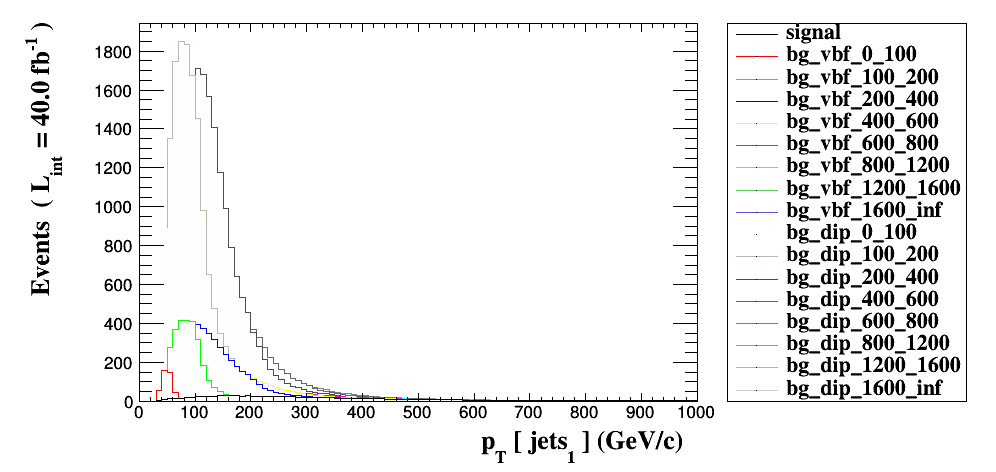
\includegraphics[scale=0.45]{selection_0.png}\\
\caption{   }
  \end{center}
\end{figure}
      \newpage
\subsection{ Histogram 2}

\textbf{* Plot: ETA ( jets[1] ) }\\
   \begin{table}[H]
  \begin{center}
    \begin{tabular}{|m{23.0mm}|m{23.0mm}|m{18.0mm}|m{19.0mm}|m{19.0mm}|m{19.0mm}|m{19.0mm}|}
      \hline
      {\cellcolor{yellow}         Dataset}& {\cellcolor{yellow}         Integral}& {\cellcolor{yellow}         Entries per event}& {\cellcolor{yellow}         Mean}& {\cellcolor{yellow}         RMS}& {\cellcolor{yellow}         \% underflow}& {\cellcolor{yellow}         \% overflow}\\
      \hline
      {\cellcolor{white}         signal}& {\cellcolor{white}         1071}& {\cellcolor{white}         1.0}& {\cellcolor{white}         -0.0081341}& {\cellcolor{white}         2.035}& {\cellcolor{red}         50.2}& {\cellcolor{red}         0.0}\\
      \hline
      {\cellcolor{white}         bg\_vbf\_0\_100}& {\cellcolor{white}         364}& {\cellcolor{white}         1.0}& {\cellcolor{white}         0.000166543}& {\cellcolor{white}         3.364}& {\cellcolor{red}         50.01}& {\cellcolor{red}         0.0}\\
      \hline
      {\cellcolor{white}         bg\_vbf\_100\_200}& {\cellcolor{white}         2253}& {\cellcolor{white}         1.0}& {\cellcolor{white}         0.00866776}& {\cellcolor{white}         2.868}& {\cellcolor{red}         49.87}& {\cellcolor{red}         0.0}\\
      \hline
      {\cellcolor{white}         bg\_vbf\_200\_400}& {\cellcolor{white}         2038}& {\cellcolor{white}         1.0}& {\cellcolor{white}         0.000566865}& {\cellcolor{white}         2.413}& {\cellcolor{red}         49.98}& {\cellcolor{red}         0.0}\\
      \hline
      {\cellcolor{white}         bg\_vbf\_400\_600}& {\cellcolor{white}         279}& {\cellcolor{white}         1.0}& {\cellcolor{white}         -0.00094651}& {\cellcolor{white}         2.161}& {\cellcolor{red}         50.04}& {\cellcolor{red}         0.0}\\
      \hline
      {\cellcolor{white}         bg\_vbf\_600\_800}& {\cellcolor{white}         47.9}& {\cellcolor{white}         1.0}& {\cellcolor{white}         -0.00189725}& {\cellcolor{white}         2.037}& {\cellcolor{red}         50.12}& {\cellcolor{red}         0.0}\\
      \hline
      {\cellcolor{white}         bg\_vbf\_800\_1200}& {\cellcolor{white}         12.1}& {\cellcolor{white}         1.0}& {\cellcolor{white}         0.00161135}& {\cellcolor{white}         1.945}& {\cellcolor{red}         49.99}& {\cellcolor{red}         0.0}\\
      \hline
      {\cellcolor{white}         bg\_vbf\_1200\_1600}& {\cellcolor{white}         0.677}& {\cellcolor{white}         1.0}& {\cellcolor{white}         -0.0110501}& {\cellcolor{white}         1.841}& {\cellcolor{red}         50.44}& {\cellcolor{red}         0.0}\\
      \hline
      {\cellcolor{white}         bg\_vbf\_1600\_inf}& {\cellcolor{white}         0.0489}& {\cellcolor{white}         1.0}& {\cellcolor{white}         0.0430261}& {\cellcolor{white}         1.762}& {\cellcolor{red}         48.57}& {\cellcolor{red}         0.0}\\
      \hline
      {\cellcolor{white}         bg\_dip\_0\_100}& {\cellcolor{white}         1767}& {\cellcolor{white}         1.0}& {\cellcolor{white}         0.00678619}& {\cellcolor{white}         3.325}& {\cellcolor{red}         50.15}& {\cellcolor{red}         0.0}\\
      \hline
      {\cellcolor{white}         bg\_dip\_100\_200}& {\cellcolor{white}         8038}& {\cellcolor{white}         1.0}& {\cellcolor{white}         0.0191145}& {\cellcolor{white}         2.85}& {\cellcolor{red}         49.76}& {\cellcolor{red}         0.0}\\
      \hline
      {\cellcolor{white}         bg\_dip\_200\_400}& {\cellcolor{white}         6955}& {\cellcolor{white}         1.0}& {\cellcolor{white}         -0.0295387}& {\cellcolor{white}         2.346}& {\cellcolor{red}         50.49}& {\cellcolor{red}         0.0}\\
      \hline
      {\cellcolor{white}         bg\_dip\_400\_600}& {\cellcolor{white}         638}& {\cellcolor{white}         1.0}& {\cellcolor{white}         -0.02202}& {\cellcolor{white}         2.092}& {\cellcolor{red}         50.52}& {\cellcolor{red}         0.0}\\
      \hline
      {\cellcolor{white}         bg\_dip\_600\_800}& {\cellcolor{white}         89.9}& {\cellcolor{white}         1.0}& {\cellcolor{white}         0.02674}& {\cellcolor{white}         2.002}& {\cellcolor{red}         49.51}& {\cellcolor{red}         0.0}\\
      \hline
      {\cellcolor{white}         bg\_dip\_800\_1200}& {\cellcolor{white}         21.9}& {\cellcolor{white}         1.0}& {\cellcolor{white}         -0.0213812}& {\cellcolor{white}         1.918}& {\cellcolor{red}         50.54}& {\cellcolor{red}         0.0}\\
      \hline
      {\cellcolor{white}         bg\_dip\_1200\_1600}& {\cellcolor{white}         1.31}& {\cellcolor{white}         1.0}& {\cellcolor{white}         0.00841074}& {\cellcolor{white}         1.835}& {\cellcolor{red}         49.89}& {\cellcolor{red}         0.0}\\
      \hline
      {\cellcolor{white}         bg\_dip\_1600\_inf}& {\cellcolor{white}         0.0878}& {\cellcolor{white}         1.0}& {\cellcolor{white}         -0.105628}& {\cellcolor{white}         1.768}& {\cellcolor{red}         53.09}& {\cellcolor{red}         0.0}\\
\hline
    \end{tabular}
  \end{center}
\end{table}

\begin{figure}[H]
  \begin{center}
    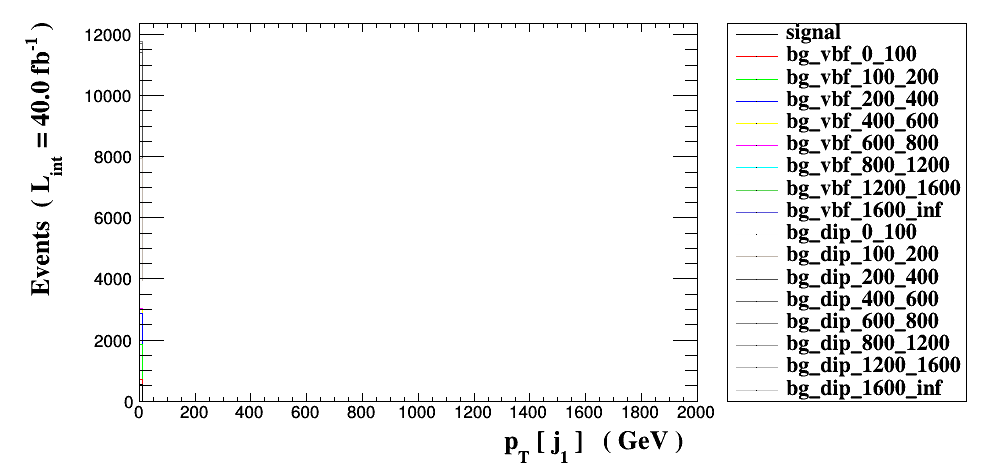
\includegraphics[scale=0.45]{selection_1.png}\\
\caption{   }
  \end{center}
\end{figure}
      \newpage
\subsection{ Histogram 3}

\textbf{* Plot: PHI ( jets[1] ) }\\
   \begin{table}[H]
  \begin{center}
    \begin{tabular}{|m{23.0mm}|m{23.0mm}|m{18.0mm}|m{19.0mm}|m{19.0mm}|m{19.0mm}|m{19.0mm}|}
      \hline
      {\cellcolor{yellow}         Dataset}& {\cellcolor{yellow}         Integral}& {\cellcolor{yellow}         Entries per event}& {\cellcolor{yellow}         Mean}& {\cellcolor{yellow}         RMS}& {\cellcolor{yellow}         \% underflow}& {\cellcolor{yellow}         \% overflow}\\
      \hline
      {\cellcolor{white}         signal}& {\cellcolor{white}         1071}& {\cellcolor{white}         1.0}& {\cellcolor{white}         -0.00110744}& {\cellcolor{white}         1.813}& {\cellcolor{green}         0.0}& {\cellcolor{green}         0.0}\\
      \hline
      {\cellcolor{white}         bg\_vbf\_0\_100}& {\cellcolor{white}         364}& {\cellcolor{white}         1.0}& {\cellcolor{white}         0.00232715}& {\cellcolor{white}         1.806}& {\cellcolor{green}         0.0}& {\cellcolor{green}         0.0}\\
      \hline
      {\cellcolor{white}         bg\_vbf\_100\_200}& {\cellcolor{white}         2253}& {\cellcolor{white}         1.0}& {\cellcolor{white}         -0.00635393}& {\cellcolor{white}         1.815}& {\cellcolor{green}         0.0}& {\cellcolor{green}         0.0}\\
      \hline
      {\cellcolor{white}         bg\_vbf\_200\_400}& {\cellcolor{white}         2038}& {\cellcolor{white}         1.0}& {\cellcolor{white}         0.00218214}& {\cellcolor{white}         1.814}& {\cellcolor{green}         0.0}& {\cellcolor{green}         0.0}\\
      \hline
      {\cellcolor{white}         bg\_vbf\_400\_600}& {\cellcolor{white}         279}& {\cellcolor{white}         1.0}& {\cellcolor{white}         -0.00497205}& {\cellcolor{white}         1.814}& {\cellcolor{green}         0.0}& {\cellcolor{green}         0.0}\\
      \hline
      {\cellcolor{white}         bg\_vbf\_600\_800}& {\cellcolor{white}         47.9}& {\cellcolor{white}         1.0}& {\cellcolor{white}         0.00410717}& {\cellcolor{white}         1.811}& {\cellcolor{green}         0.0}& {\cellcolor{green}         0.0}\\
      \hline
      {\cellcolor{white}         bg\_vbf\_800\_1200}& {\cellcolor{white}         12.1}& {\cellcolor{white}         1.0}& {\cellcolor{white}         -0.00518227}& {\cellcolor{white}         1.811}& {\cellcolor{green}         0.0}& {\cellcolor{green}         0.0}\\
      \hline
      {\cellcolor{white}         bg\_vbf\_1200\_1600}& {\cellcolor{white}         0.677}& {\cellcolor{white}         1.0}& {\cellcolor{white}         0.0259206}& {\cellcolor{white}         1.81}& {\cellcolor{green}         0.0}& {\cellcolor{green}         0.0}\\
      \hline
      {\cellcolor{white}         bg\_vbf\_1600\_inf}& {\cellcolor{white}         0.0489}& {\cellcolor{white}         1.0}& {\cellcolor{white}         -0.0500737}& {\cellcolor{white}         1.792}& {\cellcolor{green}         0.0}& {\cellcolor{green}         0.0}\\
      \hline
      {\cellcolor{white}         bg\_dip\_0\_100}& {\cellcolor{white}         1767}& {\cellcolor{white}         1.0}& {\cellcolor{white}         -0.00684135}& {\cellcolor{white}         1.756}& {\cellcolor{green}         0.0}& {\cellcolor{green}         0.0}\\
      \hline
      {\cellcolor{white}         bg\_dip\_100\_200}& {\cellcolor{white}         8038}& {\cellcolor{white}         1.0}& {\cellcolor{white}         0.0476437}& {\cellcolor{white}         1.818}& {\cellcolor{green}         0.0}& {\cellcolor{green}         0.0}\\
      \hline
      {\cellcolor{white}         bg\_dip\_200\_400}& {\cellcolor{white}         6955}& {\cellcolor{white}         1.0}& {\cellcolor{white}         -0.00756792}& {\cellcolor{white}         1.821}& {\cellcolor{green}         0.0}& {\cellcolor{green}         0.0}\\
      \hline
      {\cellcolor{white}         bg\_dip\_400\_600}& {\cellcolor{white}         638}& {\cellcolor{white}         1.0}& {\cellcolor{white}         -0.00608962}& {\cellcolor{white}         1.811}& {\cellcolor{green}         0.0}& {\cellcolor{green}         0.0}\\
      \hline
      {\cellcolor{white}         bg\_dip\_600\_800}& {\cellcolor{white}         89.9}& {\cellcolor{white}         1.0}& {\cellcolor{white}         -0.0182462}& {\cellcolor{white}         1.808}& {\cellcolor{green}         0.0}& {\cellcolor{green}         0.0}\\
      \hline
      {\cellcolor{white}         bg\_dip\_800\_1200}& {\cellcolor{white}         21.9}& {\cellcolor{white}         1.0}& {\cellcolor{white}         0.0102453}& {\cellcolor{white}         1.821}& {\cellcolor{green}         0.0}& {\cellcolor{green}         0.0}\\
      \hline
      {\cellcolor{white}         bg\_dip\_1200\_1600}& {\cellcolor{white}         1.31}& {\cellcolor{white}         1.0}& {\cellcolor{white}         -0.105508}& {\cellcolor{white}         1.774}& {\cellcolor{green}         0.0}& {\cellcolor{green}         0.0}\\
      \hline
      {\cellcolor{white}         bg\_dip\_1600\_inf}& {\cellcolor{white}         0.0878}& {\cellcolor{white}         1.0}& {\cellcolor{white}         0.042703}& {\cellcolor{white}         1.806}& {\cellcolor{green}         0.0}& {\cellcolor{green}         0.0}\\
\hline
    \end{tabular}
  \end{center}
\end{table}

\begin{figure}[H]
  \begin{center}
    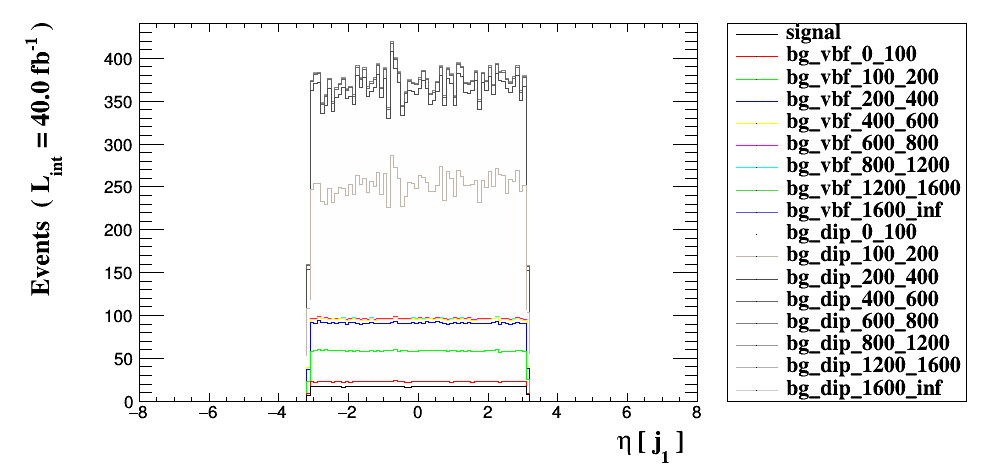
\includegraphics[scale=0.45]{selection_2.png}\\
\caption{   }
  \end{center}
\end{figure}
      \newpage
\subsection{ Histogram 4}

\textbf{* Plot: PT ( jets[2] ) }\\
   \begin{table}[H]
  \begin{center}
    \begin{tabular}{|m{23.0mm}|m{23.0mm}|m{18.0mm}|m{19.0mm}|m{19.0mm}|m{19.0mm}|m{19.0mm}|}
      \hline
      {\cellcolor{yellow}         Dataset}& {\cellcolor{yellow}         Integral}& {\cellcolor{yellow}         Entries per event}& {\cellcolor{yellow}         Mean}& {\cellcolor{yellow}         RMS}& {\cellcolor{yellow}         \% underflow}& {\cellcolor{yellow}         \% overflow}\\
      \hline
      {\cellcolor{white}         signal}& {\cellcolor{white}         1071}& {\cellcolor{white}         1.0}& {\cellcolor{white}         110.412}& {\cellcolor{white}         75.65}& {\cellcolor{red}         0.0}& {\cellcolor{red}         100.0}\\
      \hline
      {\cellcolor{white}         bg\_vbf\_0\_100}& {\cellcolor{white}         364}& {\cellcolor{white}         1.0}& {\cellcolor{white}         37.1965}& {\cellcolor{white}         4.803}& {\cellcolor{red}         0.0}& {\cellcolor{red}         100.0}\\
      \hline
      {\cellcolor{white}         bg\_vbf\_100\_200}& {\cellcolor{white}         2253}& {\cellcolor{white}         1.0}& {\cellcolor{white}         60.5597}& {\cellcolor{white}         15.75}& {\cellcolor{red}         0.0}& {\cellcolor{red}         100.0}\\
      \hline
      {\cellcolor{white}         bg\_vbf\_200\_400}& {\cellcolor{white}         2038}& {\cellcolor{white}         1.0}& {\cellcolor{white}         110.453}& {\cellcolor{white}         30.92}& {\cellcolor{red}         0.0}& {\cellcolor{red}         100.0}\\
      \hline
      {\cellcolor{white}         bg\_vbf\_400\_600}& {\cellcolor{white}         279}& {\cellcolor{white}         1.0}& {\cellcolor{white}         193.368}& {\cellcolor{white}         49.39}& {\cellcolor{red}         0.0}& {\cellcolor{red}         100.0}\\
      \hline
      {\cellcolor{white}         bg\_vbf\_600\_800}& {\cellcolor{white}         47.9}& {\cellcolor{white}         1.0}& {\cellcolor{white}         279.205}& {\cellcolor{white}         71.27}& {\cellcolor{red}         0.0}& {\cellcolor{red}         100.0}\\
      \hline
      {\cellcolor{white}         bg\_vbf\_800\_1200}& {\cellcolor{white}         12.1}& {\cellcolor{white}         1.0}& {\cellcolor{white}         380.947}& {\cellcolor{white}         107.0}& {\cellcolor{red}         0.0}& {\cellcolor{red}         100.0}\\
      \hline
      {\cellcolor{white}         bg\_vbf\_1200\_1600}& {\cellcolor{white}         0.677}& {\cellcolor{white}         1.0}& {\cellcolor{white}         550.064}& {\cellcolor{white}         164.8}& {\cellcolor{red}         0.0}& {\cellcolor{red}         100.0}\\
      \hline
      {\cellcolor{white}         bg\_vbf\_1600\_inf}& {\cellcolor{white}         0.0489}& {\cellcolor{white}         1.0}& {\cellcolor{white}         709.68}& {\cellcolor{white}         253.2}& {\cellcolor{red}         0.0}& {\cellcolor{red}         100.0}\\
      \hline
      {\cellcolor{white}         bg\_dip\_0\_100}& {\cellcolor{white}         1767}& {\cellcolor{white}         1.0}& {\cellcolor{white}         36.8168}& {\cellcolor{white}         4.657}& {\cellcolor{red}         0.0}& {\cellcolor{red}         100.0}\\
      \hline
      {\cellcolor{white}         bg\_dip\_100\_200}& {\cellcolor{white}         8038}& {\cellcolor{white}         1.0}& {\cellcolor{white}         59.3023}& {\cellcolor{white}         15.73}& {\cellcolor{red}         0.0}& {\cellcolor{red}         100.0}\\
      \hline
      {\cellcolor{white}         bg\_dip\_200\_400}& {\cellcolor{white}         6955}& {\cellcolor{white}         1.0}& {\cellcolor{white}         106.437}& {\cellcolor{white}         31.05}& {\cellcolor{red}         0.0}& {\cellcolor{red}         100.0}\\
      \hline
      {\cellcolor{white}         bg\_dip\_400\_600}& {\cellcolor{white}         638}& {\cellcolor{white}         1.0}& {\cellcolor{white}         187.342}& {\cellcolor{white}         58.65}& {\cellcolor{red}         0.0}& {\cellcolor{red}         100.0}\\
      \hline
      {\cellcolor{white}         bg\_dip\_600\_800}& {\cellcolor{white}         89.9}& {\cellcolor{white}         1.0}& {\cellcolor{white}         274.322}& {\cellcolor{white}         85.19}& {\cellcolor{red}         0.0}& {\cellcolor{red}         100.0}\\
      \hline
      {\cellcolor{white}         bg\_dip\_800\_1200}& {\cellcolor{white}         21.9}& {\cellcolor{white}         1.0}& {\cellcolor{white}         373.582}& {\cellcolor{white}         130.0}& {\cellcolor{red}         0.0}& {\cellcolor{red}         100.0}\\
      \hline
      {\cellcolor{white}         bg\_dip\_1200\_1600}& {\cellcolor{white}         1.31}& {\cellcolor{white}         1.0}& {\cellcolor{white}         557.191}& {\cellcolor{white}         176.2}& {\cellcolor{red}         0.0}& {\cellcolor{red}         100.0}\\
      \hline
      {\cellcolor{white}         bg\_dip\_1600\_inf}& {\cellcolor{white}         0.0878}& {\cellcolor{white}         1.0}& {\cellcolor{white}         735.455}& {\cellcolor{white}         261.9}& {\cellcolor{red}         0.0}& {\cellcolor{red}         100.0}\\
\hline
    \end{tabular}
  \end{center}
\end{table}

\begin{figure}[H]
  \begin{center}
    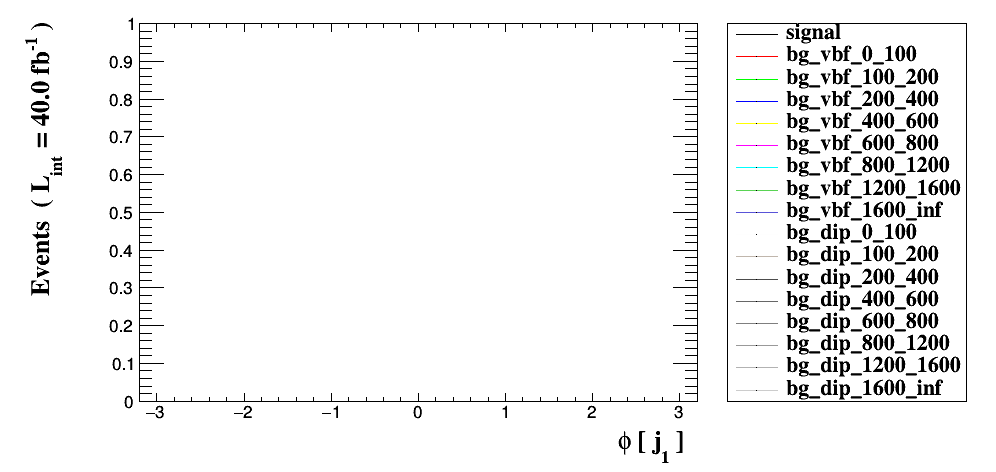
\includegraphics[scale=0.45]{selection_3.png}\\
\caption{   }
  \end{center}
\end{figure}
      \newpage
\subsection{ Histogram 5}

\textbf{* Plot: ETA ( jets[2] ) }\\
   \begin{table}[H]
  \begin{center}
    \begin{tabular}{|m{23.0mm}|m{23.0mm}|m{18.0mm}|m{19.0mm}|m{19.0mm}|m{19.0mm}|m{19.0mm}|}
      \hline
      {\cellcolor{yellow}         Dataset}& {\cellcolor{yellow}         Integral}& {\cellcolor{yellow}         Entries per event}& {\cellcolor{yellow}         Mean}& {\cellcolor{yellow}         RMS}& {\cellcolor{yellow}         \% underflow}& {\cellcolor{yellow}         \% overflow}\\
      \hline
      {\cellcolor{white}         signal}& {\cellcolor{white}         1071}& {\cellcolor{white}         1.0}& {\cellcolor{white}         0.0114933}& {\cellcolor{white}         2.943}& {\cellcolor{red}         49.8}& {\cellcolor{red}         0.0}\\
      \hline
      {\cellcolor{white}         bg\_vbf\_0\_100}& {\cellcolor{white}         364}& {\cellcolor{white}         1.0}& {\cellcolor{white}         -0.00319227}& {\cellcolor{white}         3.461}& {\cellcolor{red}         49.99}& {\cellcolor{red}         0.0}\\
      \hline
      {\cellcolor{white}         bg\_vbf\_100\_200}& {\cellcolor{white}         2253}& {\cellcolor{white}         1.0}& {\cellcolor{white}         -0.00774539}& {\cellcolor{white}         3.085}& {\cellcolor{red}         50.13}& {\cellcolor{red}         0.0}\\
      \hline
      {\cellcolor{white}         bg\_vbf\_200\_400}& {\cellcolor{white}         2038}& {\cellcolor{white}         1.0}& {\cellcolor{white}         -0.00172193}& {\cellcolor{white}         2.656}& {\cellcolor{red}         50.03}& {\cellcolor{red}         0.0}\\
      \hline
      {\cellcolor{white}         bg\_vbf\_400\_600}& {\cellcolor{white}         279}& {\cellcolor{white}         1.0}& {\cellcolor{white}         0.00254018}& {\cellcolor{white}         2.449}& {\cellcolor{red}         49.95}& {\cellcolor{red}         0.0}\\
      \hline
      {\cellcolor{white}         bg\_vbf\_600\_800}& {\cellcolor{white}         47.9}& {\cellcolor{white}         1.0}& {\cellcolor{white}         0.00692713}& {\cellcolor{white}         2.34}& {\cellcolor{red}         49.88}& {\cellcolor{red}         0.0}\\
      \hline
      {\cellcolor{white}         bg\_vbf\_800\_1200}& {\cellcolor{white}         12.1}& {\cellcolor{white}         1.0}& {\cellcolor{white}         0.000298794}& {\cellcolor{white}         2.256}& {\cellcolor{red}         50.01}& {\cellcolor{red}         0.0}\\
      \hline
      {\cellcolor{white}         bg\_vbf\_1200\_1600}& {\cellcolor{white}         0.677}& {\cellcolor{white}         1.0}& {\cellcolor{white}         0.0228384}& {\cellcolor{white}         2.194}& {\cellcolor{red}         49.56}& {\cellcolor{red}         0.0}\\
      \hline
      {\cellcolor{white}         bg\_vbf\_1600\_inf}& {\cellcolor{white}         0.0489}& {\cellcolor{white}         1.0}& {\cellcolor{white}         -0.0594671}& {\cellcolor{white}         2.201}& {\cellcolor{red}         51.32}& {\cellcolor{red}         0.0}\\
      \hline
      {\cellcolor{white}         bg\_dip\_0\_100}& {\cellcolor{white}         1767}& {\cellcolor{white}         1.0}& {\cellcolor{white}         0.0164847}& {\cellcolor{white}         3.245}& {\cellcolor{red}         49.85}& {\cellcolor{red}         0.0}\\
      \hline
      {\cellcolor{white}         bg\_dip\_100\_200}& {\cellcolor{white}         8038}& {\cellcolor{white}         1.0}& {\cellcolor{white}         -0.0159359}& {\cellcolor{white}         2.793}& {\cellcolor{red}         50.28}& {\cellcolor{red}         0.0}\\
      \hline
      {\cellcolor{white}         bg\_dip\_200\_400}& {\cellcolor{white}         6955}& {\cellcolor{white}         1.0}& {\cellcolor{white}         0.00699555}& {\cellcolor{white}         2.319}& {\cellcolor{red}         49.61}& {\cellcolor{red}         0.0}\\
      \hline
      {\cellcolor{white}         bg\_dip\_400\_600}& {\cellcolor{white}         638}& {\cellcolor{white}         1.0}& {\cellcolor{white}         0.0183088}& {\cellcolor{white}         2.263}& {\cellcolor{red}         49.54}& {\cellcolor{red}         0.0}\\
      \hline
      {\cellcolor{white}         bg\_dip\_600\_800}& {\cellcolor{white}         89.9}& {\cellcolor{white}         1.0}& {\cellcolor{white}         -0.0172787}& {\cellcolor{white}         2.223}& {\cellcolor{red}         50.52}& {\cellcolor{red}         0.0}\\
      \hline
      {\cellcolor{white}         bg\_dip\_800\_1200}& {\cellcolor{white}         21.9}& {\cellcolor{white}         1.0}& {\cellcolor{white}         0.011548}& {\cellcolor{white}         2.225}& {\cellcolor{red}         49.57}& {\cellcolor{red}         0.0}\\
      \hline
      {\cellcolor{white}         bg\_dip\_1200\_1600}& {\cellcolor{white}         1.31}& {\cellcolor{white}         1.0}& {\cellcolor{white}         0.0134887}& {\cellcolor{white}         2.165}& {\cellcolor{red}         49.88}& {\cellcolor{red}         0.0}\\
      \hline
      {\cellcolor{white}         bg\_dip\_1600\_inf}& {\cellcolor{white}         0.0878}& {\cellcolor{white}         1.0}& {\cellcolor{white}         0.114217}& {\cellcolor{white}         2.195}& {\cellcolor{red}         47.12}& {\cellcolor{red}         0.0}\\
\hline
    \end{tabular}
  \end{center}
\end{table}

\begin{figure}[H]
  \begin{center}
    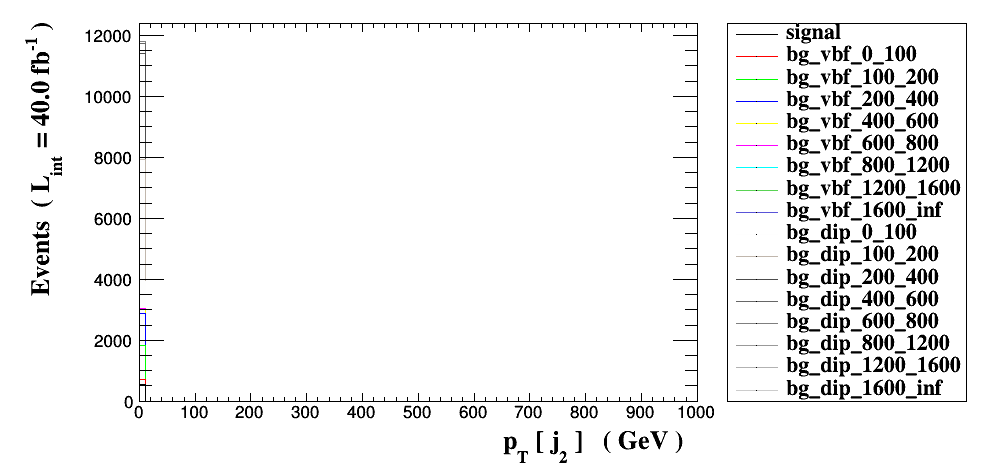
\includegraphics[scale=0.45]{selection_4.png}\\
\caption{   }
  \end{center}
\end{figure}
      \newpage
\subsection{ Histogram 6}

\textbf{* Plot: PHI ( jets[2] ) }\\
   \begin{table}[H]
  \begin{center}
    \begin{tabular}{|m{23.0mm}|m{23.0mm}|m{18.0mm}|m{19.0mm}|m{19.0mm}|m{19.0mm}|m{19.0mm}|}
      \hline
      {\cellcolor{yellow}         Dataset}& {\cellcolor{yellow}         Integral}& {\cellcolor{yellow}         Entries per event}& {\cellcolor{yellow}         Mean}& {\cellcolor{yellow}         RMS}& {\cellcolor{yellow}         \% underflow}& {\cellcolor{yellow}         \% overflow}\\
      \hline
      {\cellcolor{white}         signal}& {\cellcolor{white}         1071}& {\cellcolor{white}         1.0}& {\cellcolor{white}         -0.00115095}& {\cellcolor{white}         1.816}& {\cellcolor{green}         0.0}& {\cellcolor{green}         0.0}\\
      \hline
      {\cellcolor{white}         bg\_vbf\_0\_100}& {\cellcolor{white}         364}& {\cellcolor{white}         1.0}& {\cellcolor{white}         -0.00253582}& {\cellcolor{white}         1.816}& {\cellcolor{green}         0.0}& {\cellcolor{green}         0.0}\\
      \hline
      {\cellcolor{white}         bg\_vbf\_100\_200}& {\cellcolor{white}         2253}& {\cellcolor{white}         1.0}& {\cellcolor{white}         0.00482266}& {\cellcolor{white}         1.815}& {\cellcolor{green}         0.0}& {\cellcolor{green}         0.0}\\
      \hline
      {\cellcolor{white}         bg\_vbf\_200\_400}& {\cellcolor{white}         2038}& {\cellcolor{white}         1.0}& {\cellcolor{white}         -0.00338121}& {\cellcolor{white}         1.814}& {\cellcolor{green}         0.0}& {\cellcolor{green}         0.0}\\
      \hline
      {\cellcolor{white}         bg\_vbf\_400\_600}& {\cellcolor{white}         279}& {\cellcolor{white}         1.0}& {\cellcolor{white}         -0.000828397}& {\cellcolor{white}         1.814}& {\cellcolor{green}         0.0}& {\cellcolor{green}         0.0}\\
      \hline
      {\cellcolor{white}         bg\_vbf\_600\_800}& {\cellcolor{white}         47.9}& {\cellcolor{white}         1.0}& {\cellcolor{white}         -0.000130577}& {\cellcolor{white}         1.816}& {\cellcolor{green}         0.0}& {\cellcolor{green}         0.0}\\
      \hline
      {\cellcolor{white}         bg\_vbf\_800\_1200}& {\cellcolor{white}         12.1}& {\cellcolor{white}         1.0}& {\cellcolor{white}         -0.00939579}& {\cellcolor{white}         1.818}& {\cellcolor{green}         0.0}& {\cellcolor{green}         0.0}\\
      \hline
      {\cellcolor{white}         bg\_vbf\_1200\_1600}& {\cellcolor{white}         0.677}& {\cellcolor{white}         1.0}& {\cellcolor{white}         -0.0114353}& {\cellcolor{white}         1.817}& {\cellcolor{green}         0.0}& {\cellcolor{green}         0.0}\\
      \hline
      {\cellcolor{white}         bg\_vbf\_1600\_inf}& {\cellcolor{white}         0.0489}& {\cellcolor{white}         1.0}& {\cellcolor{white}         0.0734785}& {\cellcolor{white}         1.819}& {\cellcolor{green}         0.0}& {\cellcolor{green}         0.0}\\
      \hline
      {\cellcolor{white}         bg\_dip\_0\_100}& {\cellcolor{white}         1767}& {\cellcolor{white}         1.0}& {\cellcolor{white}         -0.0502398}& {\cellcolor{white}         1.84}& {\cellcolor{green}         0.0}& {\cellcolor{green}         0.0}\\
      \hline
      {\cellcolor{white}         bg\_dip\_100\_200}& {\cellcolor{white}         8038}& {\cellcolor{white}         1.0}& {\cellcolor{white}         0.00371512}& {\cellcolor{white}         1.806}& {\cellcolor{green}         0.0}& {\cellcolor{green}         0.0}\\
      \hline
      {\cellcolor{white}         bg\_dip\_200\_400}& {\cellcolor{white}         6955}& {\cellcolor{white}         1.0}& {\cellcolor{white}         -0.00657528}& {\cellcolor{white}         1.807}& {\cellcolor{green}         0.0}& {\cellcolor{green}         0.0}\\
      \hline
      {\cellcolor{white}         bg\_dip\_400\_600}& {\cellcolor{white}         638}& {\cellcolor{white}         1.0}& {\cellcolor{white}         -0.013669}& {\cellcolor{white}         1.819}& {\cellcolor{green}         0.0}& {\cellcolor{green}         0.0}\\
      \hline
      {\cellcolor{white}         bg\_dip\_600\_800}& {\cellcolor{white}         89.9}& {\cellcolor{white}         1.0}& {\cellcolor{white}         -0.0017161}& {\cellcolor{white}         1.819}& {\cellcolor{green}         0.0}& {\cellcolor{green}         0.0}\\
      \hline
      {\cellcolor{white}         bg\_dip\_800\_1200}& {\cellcolor{white}         21.9}& {\cellcolor{white}         1.0}& {\cellcolor{white}         0.0163775}& {\cellcolor{white}         1.808}& {\cellcolor{green}         0.0}& {\cellcolor{green}         0.0}\\
      \hline
      {\cellcolor{white}         bg\_dip\_1200\_1600}& {\cellcolor{white}         1.31}& {\cellcolor{white}         1.0}& {\cellcolor{white}         -0.0172436}& {\cellcolor{white}         1.841}& {\cellcolor{green}         0.0}& {\cellcolor{green}         0.0}\\
      \hline
      {\cellcolor{white}         bg\_dip\_1600\_inf}& {\cellcolor{white}         0.0878}& {\cellcolor{white}         1.0}& {\cellcolor{white}         -0.161061}& {\cellcolor{white}         1.828}& {\cellcolor{green}         0.0}& {\cellcolor{green}         0.0}\\
\hline
    \end{tabular}
  \end{center}
\end{table}

\begin{figure}[H]
  \begin{center}
    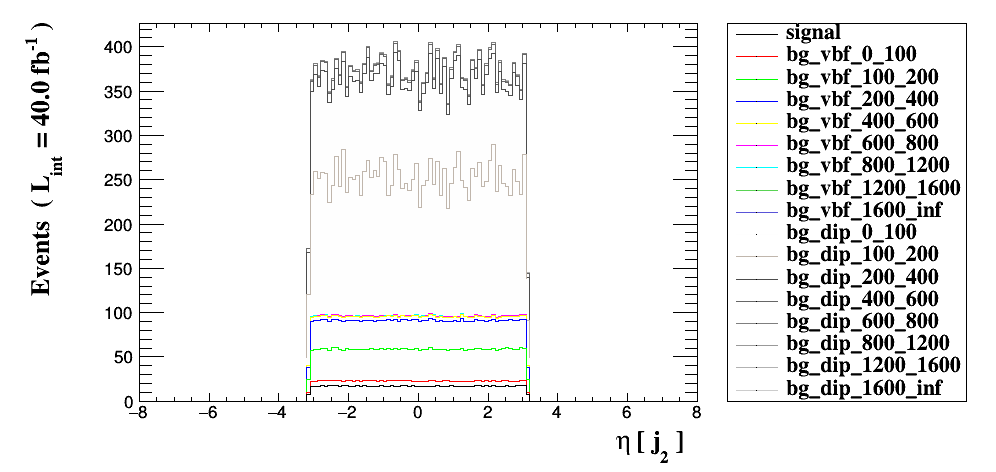
\includegraphics[scale=0.45]{selection_5.png}\\
\caption{   }
  \end{center}
\end{figure}
      \newpage
\subsection{ Histogram 7}

\textbf{* Plot: DELTAR ( jets[1] , jets[2] ) }\\
   \begin{table}[H]
  \begin{center}
    \begin{tabular}{|m{23.0mm}|m{23.0mm}|m{18.0mm}|m{19.0mm}|m{19.0mm}|m{19.0mm}|m{19.0mm}|}
      \hline
      {\cellcolor{yellow}         Dataset}& {\cellcolor{yellow}         Integral}& {\cellcolor{yellow}         Entries per event}& {\cellcolor{yellow}         Mean}& {\cellcolor{yellow}         RMS}& {\cellcolor{yellow}         \% underflow}& {\cellcolor{yellow}         \% overflow}\\
      \hline
      {\cellcolor{white}         signal}& {\cellcolor{white}         1071}& {\cellcolor{white}         1.0}& {\cellcolor{white}         5.02517}& {\cellcolor{white}         0.9314}& {\cellcolor{red}         0.0}& {\cellcolor{red}         100.0}\\
      \hline
      {\cellcolor{white}         bg\_vbf\_0\_100}& {\cellcolor{white}         364}& {\cellcolor{white}         1.0}& {\cellcolor{white}         7.05548}& {\cellcolor{white}         0.6811}& {\cellcolor{red}         0.0}& {\cellcolor{red}         100.0}\\
      \hline
      {\cellcolor{white}         bg\_vbf\_100\_200}& {\cellcolor{white}         2253}& {\cellcolor{white}         1.0}& {\cellcolor{white}         6.27976}& {\cellcolor{white}         0.7375}& {\cellcolor{red}         0.0}& {\cellcolor{red}         100.0}\\
      \hline
      {\cellcolor{white}         bg\_vbf\_200\_400}& {\cellcolor{white}         2038}& {\cellcolor{white}         1.0}& {\cellcolor{white}         5.53031}& {\cellcolor{white}         0.7056}& {\cellcolor{red}         0.0}& {\cellcolor{red}         100.0}\\
      \hline
      {\cellcolor{white}         bg\_vbf\_400\_600}& {\cellcolor{white}         279}& {\cellcolor{white}         1.0}& {\cellcolor{white}         5.226}& {\cellcolor{white}         0.5472}& {\cellcolor{red}         0.0}& {\cellcolor{red}         100.0}\\
      \hline
      {\cellcolor{white}         bg\_vbf\_600\_800}& {\cellcolor{white}         47.9}& {\cellcolor{white}         1.0}& {\cellcolor{white}         5.08807}& {\cellcolor{white}         0.4506}& {\cellcolor{red}         0.0}& {\cellcolor{red}         100.0}\\
      \hline
      {\cellcolor{white}         bg\_vbf\_800\_1200}& {\cellcolor{white}         12.1}& {\cellcolor{white}         1.0}& {\cellcolor{white}         4.98333}& {\cellcolor{white}         0.3753}& {\cellcolor{red}         0.0}& {\cellcolor{red}         100.0}\\
      \hline
      {\cellcolor{white}         bg\_vbf\_1200\_1600}& {\cellcolor{white}         0.677}& {\cellcolor{white}         1.0}& {\cellcolor{white}         4.88035}& {\cellcolor{white}         0.3011}& {\cellcolor{red}         0.0}& {\cellcolor{red}         100.0}\\
      \hline
      {\cellcolor{white}         bg\_vbf\_1600\_inf}& {\cellcolor{white}         0.0489}& {\cellcolor{white}         1.0}& {\cellcolor{white}         4.81922}& {\cellcolor{white}         0.2711}& {\cellcolor{red}         0.0}& {\cellcolor{red}         100.0}\\
      \hline
      {\cellcolor{white}         bg\_dip\_0\_100}& {\cellcolor{white}         1767}& {\cellcolor{white}         1.0}& {\cellcolor{white}         6.70448}& {\cellcolor{white}         0.4505}& {\cellcolor{red}         0.0}& {\cellcolor{red}         100.0}\\
      \hline
      {\cellcolor{white}         bg\_dip\_100\_200}& {\cellcolor{white}         8038}& {\cellcolor{white}         1.0}& {\cellcolor{white}         5.87967}& {\cellcolor{white}         0.5235}& {\cellcolor{red}         0.0}& {\cellcolor{red}         100.0}\\
      \hline
      {\cellcolor{white}         bg\_dip\_200\_400}& {\cellcolor{white}         6955}& {\cellcolor{white}         1.0}& {\cellcolor{white}         5.11228}& {\cellcolor{white}         0.4519}& {\cellcolor{red}         0.0}& {\cellcolor{red}         100.0}\\
      \hline
      {\cellcolor{white}         bg\_dip\_400\_600}& {\cellcolor{white}         638}& {\cellcolor{white}         1.0}& {\cellcolor{white}         4.96626}& {\cellcolor{white}         0.3974}& {\cellcolor{red}         0.0}& {\cellcolor{red}         100.0}\\
      \hline
      {\cellcolor{white}         bg\_dip\_600\_800}& {\cellcolor{white}         89.9}& {\cellcolor{white}         1.0}& {\cellcolor{white}         4.92962}& {\cellcolor{white}         0.349}& {\cellcolor{red}         0.0}& {\cellcolor{red}         100.0}\\
      \hline
      {\cellcolor{white}         bg\_dip\_800\_1200}& {\cellcolor{white}         21.9}& {\cellcolor{white}         1.0}& {\cellcolor{white}         4.89533}& {\cellcolor{white}         0.3164}& {\cellcolor{red}         0.0}& {\cellcolor{red}         100.0}\\
      \hline
      {\cellcolor{white}         bg\_dip\_1200\_1600}& {\cellcolor{white}         1.31}& {\cellcolor{white}         1.0}& {\cellcolor{white}         4.83455}& {\cellcolor{white}         0.2742}& {\cellcolor{red}         0.0}& {\cellcolor{red}         100.0}\\
      \hline
      {\cellcolor{white}         bg\_dip\_1600\_inf}& {\cellcolor{white}         0.0878}& {\cellcolor{white}         1.0}& {\cellcolor{white}         4.81616}& {\cellcolor{white}         0.2395}& {\cellcolor{red}         0.0}& {\cellcolor{red}         100.0}\\
\hline
    \end{tabular}
  \end{center}
\end{table}

\begin{figure}[H]
  \begin{center}
    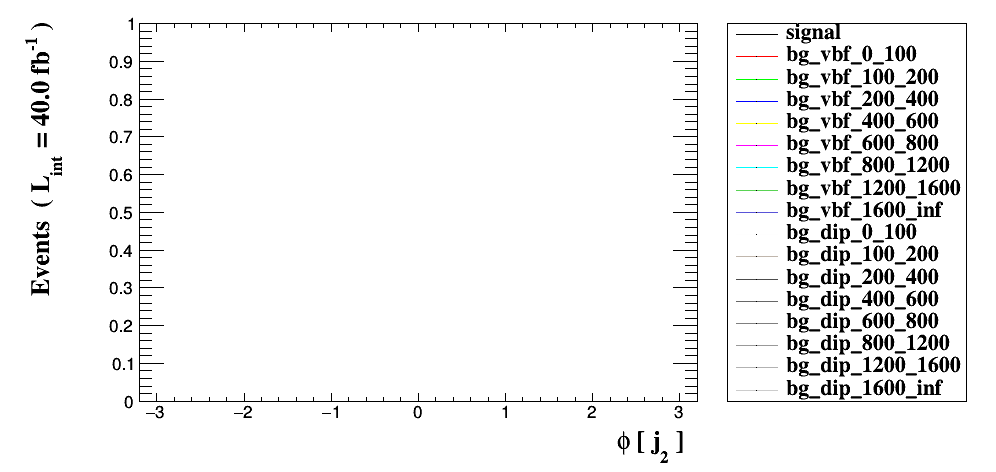
\includegraphics[scale=0.45]{selection_6.png}\\
\caption{   }
  \end{center}
\end{figure}
      \newpage
\subsection{ Histogram 8}

\textbf{* Plot: M ( jets[1] jets[2] ) }\\
   \begin{table}[H]
  \begin{center}
    \begin{tabular}{|m{23.0mm}|m{23.0mm}|m{18.0mm}|m{19.0mm}|m{19.0mm}|m{19.0mm}|m{19.0mm}|}
      \hline
      {\cellcolor{yellow}         Dataset}& {\cellcolor{yellow}         Integral}& {\cellcolor{yellow}         Entries per event}& {\cellcolor{yellow}         Mean}& {\cellcolor{yellow}         RMS}& {\cellcolor{yellow}         \% underflow}& {\cellcolor{yellow}         \% overflow}\\
      \hline
      {\cellcolor{white}         signal}& {\cellcolor{white}         1071}& {\cellcolor{white}         1.0}& {\cellcolor{white}         1782.84}& {\cellcolor{white}         805.6}& {\cellcolor{red}         0.0}& {\cellcolor{red}         100.0}\\
      \hline
      {\cellcolor{white}         bg\_vbf\_0\_100}& {\cellcolor{white}         364}& {\cellcolor{white}         1.0}& {\cellcolor{white}         1218.46}& {\cellcolor{white}         518.8}& {\cellcolor{red}         0.0}& {\cellcolor{red}         100.0}\\
      \hline
      {\cellcolor{white}         bg\_vbf\_100\_200}& {\cellcolor{white}         2253}& {\cellcolor{white}         1.0}& {\cellcolor{white}         1300.68}& {\cellcolor{white}         563.7}& {\cellcolor{red}         0.0}& {\cellcolor{red}         100.0}\\
      \hline
      {\cellcolor{white}         bg\_vbf\_200\_400}& {\cellcolor{white}         2038}& {\cellcolor{white}         1.0}& {\cellcolor{white}         1525.14}& {\cellcolor{white}         681.4}& {\cellcolor{red}         0.0}& {\cellcolor{red}         100.0}\\
      \hline
      {\cellcolor{white}         bg\_vbf\_400\_600}& {\cellcolor{white}         279}& {\cellcolor{white}         1.0}& {\cellcolor{white}         2158.83}& {\cellcolor{white}         747.9}& {\cellcolor{red}         0.0}& {\cellcolor{red}         100.0}\\
      \hline
      {\cellcolor{white}         bg\_vbf\_600\_800}& {\cellcolor{white}         47.9}& {\cellcolor{white}         1.0}& {\cellcolor{white}         2776.13}& {\cellcolor{white}         765.8}& {\cellcolor{red}         0.0}& {\cellcolor{red}         100.0}\\
      \hline
      {\cellcolor{white}         bg\_vbf\_800\_1200}& {\cellcolor{white}         12.1}& {\cellcolor{white}         1.0}& {\cellcolor{white}         3449.71}& {\cellcolor{white}         798.9}& {\cellcolor{red}         0.0}& {\cellcolor{red}         100.0}\\
      \hline
      {\cellcolor{white}         bg\_vbf\_1200\_1600}& {\cellcolor{white}         0.677}& {\cellcolor{white}         1.0}& {\cellcolor{white}         4539.84}& {\cellcolor{white}         866.7}& {\cellcolor{red}         0.0}& {\cellcolor{red}         100.0}\\
      \hline
      {\cellcolor{white}         bg\_vbf\_1600\_inf}& {\cellcolor{white}         0.0489}& {\cellcolor{white}         1.0}& {\cellcolor{white}         5592.0}& {\cellcolor{white}         1139}& {\cellcolor{red}         0.0}& {\cellcolor{red}         100.0}\\
      \hline
      {\cellcolor{white}         bg\_dip\_0\_100}& {\cellcolor{white}         1767}& {\cellcolor{white}         1.0}& {\cellcolor{white}         941.446}& {\cellcolor{white}         217.6}& {\cellcolor{red}         0.0}& {\cellcolor{red}         100.0}\\
      \hline
      {\cellcolor{white}         bg\_dip\_100\_200}& {\cellcolor{white}         8038}& {\cellcolor{white}         1.0}& {\cellcolor{white}         977.574}& {\cellcolor{white}         247.5}& {\cellcolor{red}         0.0}& {\cellcolor{red}         100.0}\\
      \hline
      {\cellcolor{white}         bg\_dip\_200\_400}& {\cellcolor{white}         6955}& {\cellcolor{white}         1.0}& {\cellcolor{white}         1100.31}& {\cellcolor{white}         326.2}& {\cellcolor{red}         0.0}& {\cellcolor{red}         100.0}\\
      \hline
      {\cellcolor{white}         bg\_dip\_400\_600}& {\cellcolor{white}         638}& {\cellcolor{white}         1.0}& {\cellcolor{white}         1740.23}& {\cellcolor{white}         454.6}& {\cellcolor{red}         0.0}& {\cellcolor{red}         100.0}\\
      \hline
      {\cellcolor{white}         bg\_dip\_600\_800}& {\cellcolor{white}         89.9}& {\cellcolor{white}         1.0}& {\cellcolor{white}         2400.64}& {\cellcolor{white}         565.0}& {\cellcolor{red}         0.0}& {\cellcolor{red}         100.0}\\
      \hline
      {\cellcolor{white}         bg\_dip\_800\_1200}& {\cellcolor{white}         21.9}& {\cellcolor{white}         1.0}& {\cellcolor{white}         3115.39}& {\cellcolor{white}         733.4}& {\cellcolor{red}         0.0}& {\cellcolor{red}         100.0}\\
      \hline
      {\cellcolor{white}         bg\_dip\_1200\_1600}& {\cellcolor{white}         1.31}& {\cellcolor{white}         1.0}& {\cellcolor{white}         4291.95}& {\cellcolor{white}         869.7}& {\cellcolor{red}         0.0}& {\cellcolor{red}         100.0}\\
      \hline
      {\cellcolor{white}         bg\_dip\_1600\_inf}& {\cellcolor{white}         0.0878}& {\cellcolor{white}         1.0}& {\cellcolor{white}         5430.07}& {\cellcolor{white}         1224}& {\cellcolor{red}         0.0}& {\cellcolor{red}         100.0}\\
\hline
    \end{tabular}
  \end{center}
\end{table}

\begin{figure}[H]
  \begin{center}
    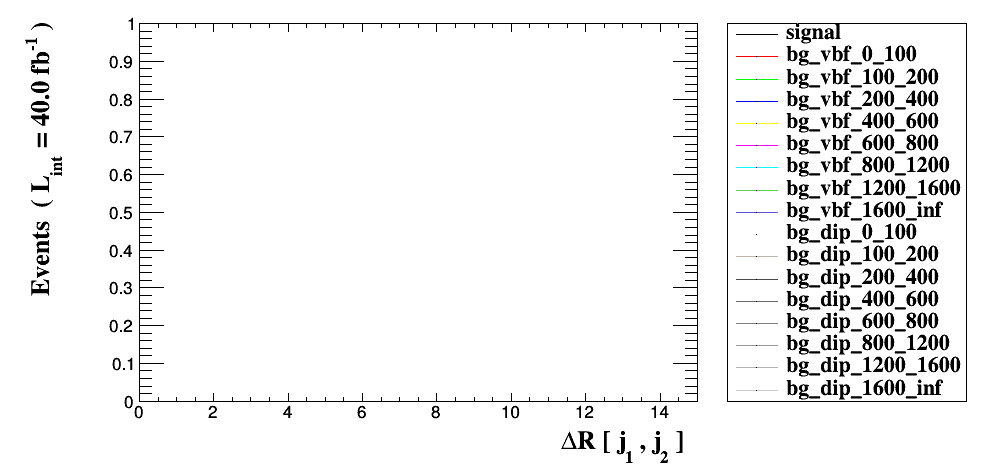
\includegraphics[scale=0.45]{selection_7.png}\\
\caption{   }
  \end{center}
\end{figure}
      \newpage
\subsection{ Histogram 9}

\textbf{* Plot: sdETA ( jets[1] jets[2] ) }\\
   \begin{table}[H]
  \begin{center}
    \begin{tabular}{|m{23.0mm}|m{23.0mm}|m{18.0mm}|m{19.0mm}|m{19.0mm}|m{19.0mm}|m{19.0mm}|}
      \hline
      {\cellcolor{yellow}         Dataset}& {\cellcolor{yellow}         Integral}& {\cellcolor{yellow}         Entries per event}& {\cellcolor{yellow}         Mean}& {\cellcolor{yellow}         RMS}& {\cellcolor{yellow}         \% underflow}& {\cellcolor{yellow}         \% overflow}\\
      \hline
      {\cellcolor{white}         signal}& {\cellcolor{white}         1071}& {\cellcolor{white}         1.0}& {\cellcolor{white}         -0.0196274}& {\cellcolor{white}         4.775}& {\cellcolor{green}         0.3136}& {\cellcolor{green}         0.0}\\
      \hline
      {\cellcolor{white}         bg\_vbf\_0\_100}& {\cellcolor{white}         364}& {\cellcolor{white}         1.0}& {\cellcolor{white}         0.00335882}& {\cellcolor{white}         6.627}& {\cellcolor{green}         2.362}& {\cellcolor{green}         0.0}\\
      \hline
      {\cellcolor{white}         bg\_vbf\_100\_200}& {\cellcolor{white}         2253}& {\cellcolor{white}         1.0}& {\cellcolor{white}         0.0164131}& {\cellcolor{white}         5.726}& {\cellcolor{green}         0.3636}& {\cellcolor{green}         0.0}\\
      \hline
      {\cellcolor{white}         bg\_vbf\_200\_400}& {\cellcolor{white}         2038}& {\cellcolor{white}         1.0}& {\cellcolor{white}         0.0022888}& {\cellcolor{white}         4.839}& {\cellcolor{green}         0.01241}& {\cellcolor{green}         0.0}\\
      \hline
      {\cellcolor{white}         bg\_vbf\_400\_600}& {\cellcolor{white}         279}& {\cellcolor{white}         1.0}& {\cellcolor{white}         -0.00348669}& {\cellcolor{white}         4.443}& {\cellcolor{green}         0.0}& {\cellcolor{green}         0.0}\\
      \hline
      {\cellcolor{white}         bg\_vbf\_600\_800}& {\cellcolor{white}         47.9}& {\cellcolor{white}         1.0}& {\cellcolor{white}         -0.00882439}& {\cellcolor{white}         4.247}& {\cellcolor{green}         0.0}& {\cellcolor{green}         0.0}\\
      \hline
      {\cellcolor{white}         bg\_vbf\_800\_1200}& {\cellcolor{white}         12.1}& {\cellcolor{white}         1.0}& {\cellcolor{white}         0.00131256}& {\cellcolor{white}         4.094}& {\cellcolor{green}         0.0}& {\cellcolor{green}         0.0}\\
      \hline
      {\cellcolor{white}         bg\_vbf\_1200\_1600}& {\cellcolor{white}         0.677}& {\cellcolor{white}         1.0}& {\cellcolor{white}         -0.0338885}& {\cellcolor{white}         3.938}& {\cellcolor{green}         0.0}& {\cellcolor{green}         0.0}\\
      \hline
      {\cellcolor{white}         bg\_vbf\_1600\_inf}& {\cellcolor{white}         0.0489}& {\cellcolor{white}         1.0}& {\cellcolor{white}         0.102493}& {\cellcolor{white}         3.852}& {\cellcolor{green}         0.0}& {\cellcolor{green}         0.0}\\
      \hline
      {\cellcolor{white}         bg\_dip\_0\_100}& {\cellcolor{white}         1767}& {\cellcolor{white}         1.0}& {\cellcolor{white}         -0.0096985}& {\cellcolor{white}         6.187}& {\cellcolor{green}         0.0}& {\cellcolor{green}         0.0}\\
      \hline
      {\cellcolor{white}         bg\_dip\_100\_200}& {\cellcolor{white}         8038}& {\cellcolor{white}         1.0}& {\cellcolor{white}         0.0350504}& {\cellcolor{white}         5.238}& {\cellcolor{green}         0.0}& {\cellcolor{green}         0.0}\\
      \hline
      {\cellcolor{white}         bg\_dip\_200\_400}& {\cellcolor{white}         6955}& {\cellcolor{white}         1.0}& {\cellcolor{white}         -0.0365342}& {\cellcolor{white}         4.29}& {\cellcolor{green}         0.0}& {\cellcolor{green}         0.0}\\
      \hline
      {\cellcolor{white}         bg\_dip\_400\_600}& {\cellcolor{white}         638}& {\cellcolor{white}         1.0}& {\cellcolor{white}         -0.0403288}& {\cellcolor{white}         4.085}& {\cellcolor{green}         0.0}& {\cellcolor{green}         0.0}\\
      \hline
      {\cellcolor{white}         bg\_dip\_600\_800}& {\cellcolor{white}         89.9}& {\cellcolor{white}         1.0}& {\cellcolor{white}         0.0440187}& {\cellcolor{white}         4.012}& {\cellcolor{green}         0.0}& {\cellcolor{green}         0.0}\\
      \hline
      {\cellcolor{white}         bg\_dip\_800\_1200}& {\cellcolor{white}         21.9}& {\cellcolor{white}         1.0}& {\cellcolor{white}         -0.0329292}& {\cellcolor{white}         3.953}& {\cellcolor{green}         0.0}& {\cellcolor{green}         0.0}\\
      \hline
      {\cellcolor{white}         bg\_dip\_1200\_1600}& {\cellcolor{white}         1.31}& {\cellcolor{white}         1.0}& {\cellcolor{white}         -0.00507792}& {\cellcolor{white}         3.851}& {\cellcolor{green}         0.0}& {\cellcolor{green}         0.0}\\
      \hline
      {\cellcolor{white}         bg\_dip\_1600\_inf}& {\cellcolor{white}         0.0878}& {\cellcolor{white}         1.0}& {\cellcolor{white}         -0.219844}& {\cellcolor{white}         3.802}& {\cellcolor{green}         0.0}& {\cellcolor{green}         0.0}\\
\hline
    \end{tabular}
  \end{center}
\end{table}

\begin{figure}[H]
  \begin{center}
    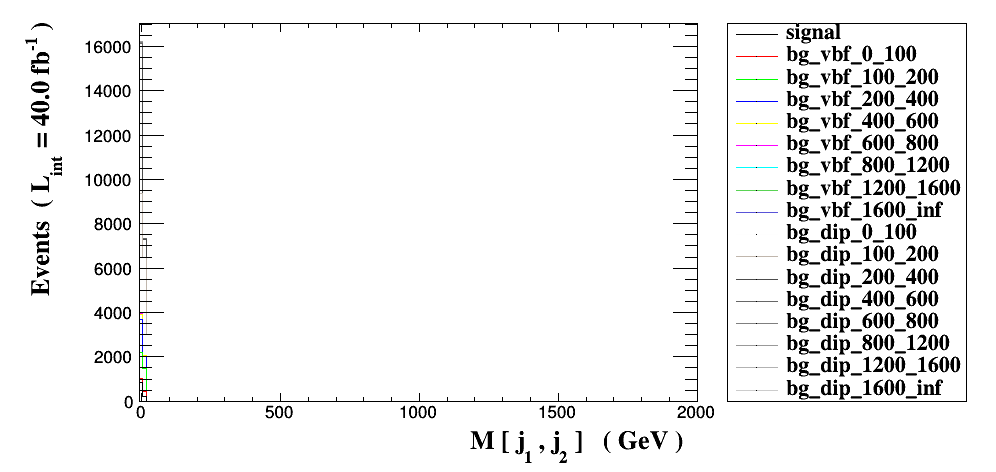
\includegraphics[scale=0.45]{selection_8.png}\\
\caption{   }
  \end{center}
\end{figure}
      \newpage
\subsection{ Histogram 10}

\textbf{* Plot: M ( a[1] a[2] ) }\\
   \begin{table}[H]
  \begin{center}
    \begin{tabular}{|m{23.0mm}|m{23.0mm}|m{18.0mm}|m{19.0mm}|m{19.0mm}|m{19.0mm}|m{19.0mm}|}
      \hline
      {\cellcolor{yellow}         Dataset}& {\cellcolor{yellow}         Integral}& {\cellcolor{yellow}         Entries per event}& {\cellcolor{yellow}         Mean}& {\cellcolor{yellow}         RMS}& {\cellcolor{yellow}         \% underflow}& {\cellcolor{yellow}         \% overflow}\\
      \hline
      {\cellcolor{white}         signal}& {\cellcolor{white}         1071}& {\cellcolor{white}         1.0}& {\cellcolor{white}         1011.28}& {\cellcolor{white}         775.8}& {\cellcolor{red}         0.00191}& {\cellcolor{red}         99.98}\\
      \hline
      {\cellcolor{white}         bg\_vbf\_0\_100}& {\cellcolor{white}         364}& {\cellcolor{white}         1.0}& {\cellcolor{white}         68.7677}& {\cellcolor{white}         58.89}& {\cellcolor{red}         0.0}& {\cellcolor{red}         99.51}\\
      \hline
      {\cellcolor{white}         bg\_vbf\_100\_200}& {\cellcolor{white}         2253}& {\cellcolor{white}         1.0}& {\cellcolor{white}         82.8463}& {\cellcolor{white}         76.05}& {\cellcolor{red}         0.0}& {\cellcolor{red}         99.65}\\
      \hline
      {\cellcolor{white}         bg\_vbf\_200\_400}& {\cellcolor{white}         2038}& {\cellcolor{white}         1.0}& {\cellcolor{white}         106.688}& {\cellcolor{white}         106.2}& {\cellcolor{red}         0.0}& {\cellcolor{red}         99.78}\\
      \hline
      {\cellcolor{white}         bg\_vbf\_400\_600}& {\cellcolor{white}         279}& {\cellcolor{white}         1.0}& {\cellcolor{white}         142.045}& {\cellcolor{white}         146.8}& {\cellcolor{red}         0.0}& {\cellcolor{red}         99.84}\\
      \hline
      {\cellcolor{white}         bg\_vbf\_600\_800}& {\cellcolor{white}         47.9}& {\cellcolor{white}         1.0}& {\cellcolor{white}         166.359}& {\cellcolor{white}         177.6}& {\cellcolor{red}         0.0}& {\cellcolor{red}         99.89}\\
      \hline
      {\cellcolor{white}         bg\_vbf\_800\_1200}& {\cellcolor{white}         12.1}& {\cellcolor{white}         1.0}& {\cellcolor{white}         185.02}& {\cellcolor{white}         201.3}& {\cellcolor{red}         0.0}& {\cellcolor{red}         99.83}\\
      \hline
      {\cellcolor{white}         bg\_vbf\_1200\_1600}& {\cellcolor{white}         0.677}& {\cellcolor{white}         1.0}& {\cellcolor{white}         212.298}& {\cellcolor{white}         241.3}& {\cellcolor{red}         0.0}& {\cellcolor{red}         99.91}\\
      \hline
      {\cellcolor{white}         bg\_vbf\_1600\_inf}& {\cellcolor{white}         0.0489}& {\cellcolor{white}         1.0}& {\cellcolor{white}         250.072}& {\cellcolor{white}         300.4}& {\cellcolor{red}         0.0}& {\cellcolor{red}         100.0}\\
      \hline
      {\cellcolor{white}         bg\_dip\_0\_100}& {\cellcolor{white}         1767}& {\cellcolor{white}         1.0}& {\cellcolor{white}         55.0914}& {\cellcolor{white}         49.81}& {\cellcolor{red}         0.0}& {\cellcolor{red}         98.38}\\
      \hline
      {\cellcolor{white}         bg\_dip\_100\_200}& {\cellcolor{white}         8038}& {\cellcolor{white}         1.0}& {\cellcolor{white}         72.9642}& {\cellcolor{white}         79.79}& {\cellcolor{red}         0.0}& {\cellcolor{red}         99.12}\\
      \hline
      {\cellcolor{white}         bg\_dip\_200\_400}& {\cellcolor{white}         6955}& {\cellcolor{white}         1.0}& {\cellcolor{white}         94.8297}& {\cellcolor{white}         109.3}& {\cellcolor{red}         0.0}& {\cellcolor{red}         99.35}\\
      \hline
      {\cellcolor{white}         bg\_dip\_400\_600}& {\cellcolor{white}         638}& {\cellcolor{white}         1.0}& {\cellcolor{white}         137.775}& {\cellcolor{white}         161.9}& {\cellcolor{red}         0.0}& {\cellcolor{red}         99.6}\\
      \hline
      {\cellcolor{white}         bg\_dip\_600\_800}& {\cellcolor{white}         89.9}& {\cellcolor{white}         1.0}& {\cellcolor{white}         166.248}& {\cellcolor{white}         201.7}& {\cellcolor{red}         0.0}& {\cellcolor{red}         99.69}\\
      \hline
      {\cellcolor{white}         bg\_dip\_800\_1200}& {\cellcolor{white}         21.9}& {\cellcolor{white}         1.0}& {\cellcolor{white}         192.898}& {\cellcolor{white}         232.4}& {\cellcolor{red}         0.0}& {\cellcolor{red}         99.75}\\
      \hline
      {\cellcolor{white}         bg\_dip\_1200\_1600}& {\cellcolor{white}         1.31}& {\cellcolor{white}         1.0}& {\cellcolor{white}         219.777}& {\cellcolor{white}         285.3}& {\cellcolor{red}         0.0}& {\cellcolor{red}         99.77}\\
      \hline
      {\cellcolor{white}         bg\_dip\_1600\_inf}& {\cellcolor{white}         0.0878}& {\cellcolor{white}         1.0}& {\cellcolor{white}         250.056}& {\cellcolor{white}         289.6}& {\cellcolor{red}         0.0}& {\cellcolor{red}         100.0}\\
\hline
    \end{tabular}
  \end{center}
\end{table}

\begin{figure}[H]
  \begin{center}
    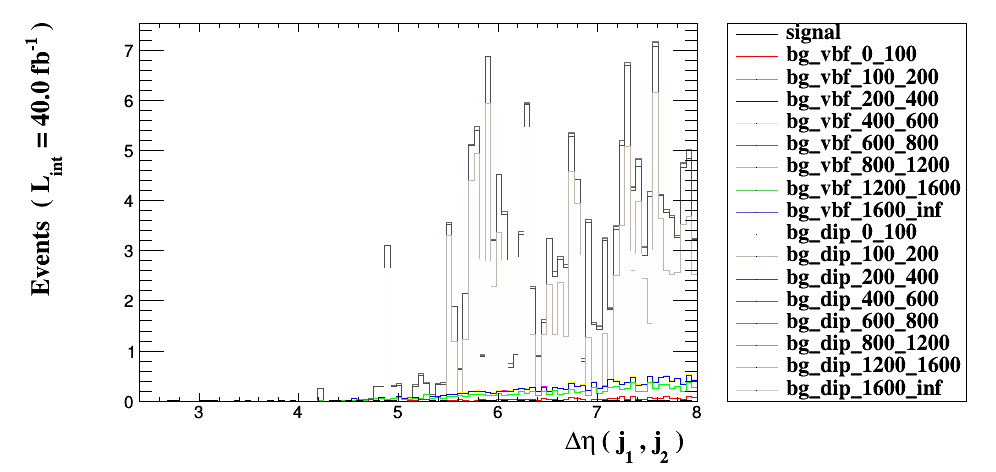
\includegraphics[scale=0.45]{selection_9.png}\\
\caption{   }
  \end{center}
\end{figure}
      \newpage
\subsection{ Histogram 11}

\textbf{* Plot: PT ( a[1] ) }\\
   \begin{table}[H]
  \begin{center}
    \begin{tabular}{|m{23.0mm}|m{23.0mm}|m{18.0mm}|m{19.0mm}|m{19.0mm}|m{19.0mm}|m{19.0mm}|}
      \hline
      {\cellcolor{yellow}         Dataset}& {\cellcolor{yellow}         Integral}& {\cellcolor{yellow}         Entries per event}& {\cellcolor{yellow}         Mean}& {\cellcolor{yellow}         RMS}& {\cellcolor{yellow}         \% underflow}& {\cellcolor{yellow}         \% overflow}\\
      \hline
      {\cellcolor{white}         signal}& {\cellcolor{white}         1071}& {\cellcolor{white}         1.0}& {\cellcolor{white}         560.533}& {\cellcolor{white}         359.9}& {\cellcolor{orange}         0.0}& {\cellcolor{orange}         11.28}\\
      \hline
      {\cellcolor{white}         bg\_vbf\_0\_100}& {\cellcolor{white}         364}& {\cellcolor{white}         1.0}& {\cellcolor{white}         34.8674}& {\cellcolor{white}         20.89}& {\cellcolor{green}         0.0}& {\cellcolor{green}         0.0}\\
      \hline
      {\cellcolor{white}         bg\_vbf\_100\_200}& {\cellcolor{white}         2253}& {\cellcolor{white}         1.0}& {\cellcolor{white}         48.7591}& {\cellcolor{white}         32.63}& {\cellcolor{green}         0.0}& {\cellcolor{green}         0.0}\\
      \hline
      {\cellcolor{white}         bg\_vbf\_200\_400}& {\cellcolor{white}         2038}& {\cellcolor{white}         1.0}& {\cellcolor{white}         76.5836}& {\cellcolor{white}         62.39}& {\cellcolor{green}         0.0}& {\cellcolor{green}         0.0005396}\\
      \hline
      {\cellcolor{white}         bg\_vbf\_400\_600}& {\cellcolor{white}         279}& {\cellcolor{white}         1.0}& {\cellcolor{white}         124.042}& {\cellcolor{white}         113.6}& {\cellcolor{green}         0.0}& {\cellcolor{green}         0.004942}\\
      \hline
      {\cellcolor{white}         bg\_vbf\_600\_800}& {\cellcolor{white}         47.9}& {\cellcolor{white}         1.0}& {\cellcolor{white}         163.938}& {\cellcolor{white}         164.9}& {\cellcolor{green}         0.0}& {\cellcolor{green}         0.01894}\\
      \hline
      {\cellcolor{white}         bg\_vbf\_800\_1200}& {\cellcolor{white}         12.1}& {\cellcolor{white}         1.0}& {\cellcolor{white}         206.18}& {\cellcolor{white}         230.8}& {\cellcolor{green}         0.0}& {\cellcolor{green}         0.688}\\
      \hline
      {\cellcolor{white}         bg\_vbf\_1200\_1600}& {\cellcolor{white}         0.677}& {\cellcolor{white}         1.0}& {\cellcolor{white}         275.804}& {\cellcolor{white}         350.4}& {\cellcolor{orange}         0.0}& {\cellcolor{orange}         8.138}\\
      \hline
      {\cellcolor{white}         bg\_vbf\_1600\_inf}& {\cellcolor{white}         0.0489}& {\cellcolor{white}         1.0}& {\cellcolor{white}         390.518}& {\cellcolor{white}         544.5}& {\cellcolor{red}         0.0}& {\cellcolor{red}         15.49}\\
      \hline
      {\cellcolor{white}         bg\_dip\_0\_100}& {\cellcolor{white}         1767}& {\cellcolor{white}         1.0}& {\cellcolor{white}         33.9862}& {\cellcolor{white}         21.96}& {\cellcolor{green}         0.0}& {\cellcolor{green}         0.0}\\
      \hline
      {\cellcolor{white}         bg\_dip\_100\_200}& {\cellcolor{white}         8038}& {\cellcolor{white}         1.0}& {\cellcolor{white}         49.2095}& {\cellcolor{white}         37.35}& {\cellcolor{green}         0.0}& {\cellcolor{green}         0.0}\\
      \hline
      {\cellcolor{white}         bg\_dip\_200\_400}& {\cellcolor{white}         6955}& {\cellcolor{white}         1.0}& {\cellcolor{white}         72.5124}& {\cellcolor{white}         67.5}& {\cellcolor{green}         0.0}& {\cellcolor{green}         0.0}\\
      \hline
      {\cellcolor{white}         bg\_dip\_400\_600}& {\cellcolor{white}         638}& {\cellcolor{white}         1.0}& {\cellcolor{white}         120.275}& {\cellcolor{white}         129.7}& {\cellcolor{green}         0.0}& {\cellcolor{green}         0.0}\\
      \hline
      {\cellcolor{white}         bg\_dip\_600\_800}& {\cellcolor{white}         89.9}& {\cellcolor{white}         1.0}& {\cellcolor{white}         154.217}& {\cellcolor{white}         184.2}& {\cellcolor{green}         0.0}& {\cellcolor{green}         0.02244}\\
      \hline
      {\cellcolor{white}         bg\_dip\_800\_1200}& {\cellcolor{white}         21.9}& {\cellcolor{white}         1.0}& {\cellcolor{white}         198.244}& {\cellcolor{white}         267.4}& {\cellcolor{green}         0.0}& {\cellcolor{green}         1.657}\\
      \hline
      {\cellcolor{white}         bg\_dip\_1200\_1600}& {\cellcolor{white}         1.31}& {\cellcolor{white}         1.0}& {\cellcolor{white}         236.703}& {\cellcolor{white}         375.1}& {\cellcolor{orange}         0.0}& {\cellcolor{orange}         9.51}\\
      \hline
      {\cellcolor{white}         bg\_dip\_1600\_inf}& {\cellcolor{white}         0.0878}& {\cellcolor{white}         1.0}& {\cellcolor{white}         309.098}& {\cellcolor{white}         544.6}& {\cellcolor{orange}         0.0}& {\cellcolor{orange}         12.35}\\
\hline
    \end{tabular}
  \end{center}
\end{table}

\begin{figure}[H]
  \begin{center}
    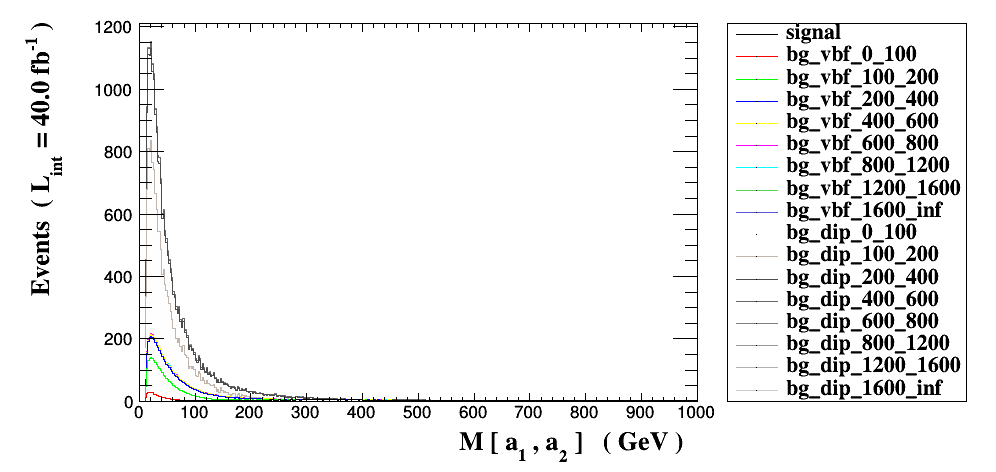
\includegraphics[scale=0.45]{selection_10.png}\\
\caption{   }
  \end{center}
\end{figure}
      \newpage
\subsection{ Histogram 12}

\textbf{* Plot: PT ( a[2] ) }\\
   \begin{table}[H]
  \begin{center}
    \begin{tabular}{|m{23.0mm}|m{23.0mm}|m{18.0mm}|m{19.0mm}|m{19.0mm}|m{19.0mm}|m{19.0mm}|}
      \hline
      {\cellcolor{yellow}         Dataset}& {\cellcolor{yellow}         Integral}& {\cellcolor{yellow}         Entries per event}& {\cellcolor{yellow}         Mean}& {\cellcolor{yellow}         RMS}& {\cellcolor{yellow}         \% underflow}& {\cellcolor{yellow}         \% overflow}\\
      \hline
      {\cellcolor{white}         signal}& {\cellcolor{white}         1071}& {\cellcolor{white}         1.0}& {\cellcolor{white}         354.913}& {\cellcolor{white}         315.1}& {\cellcolor{green}         0.0}& {\cellcolor{green}         4.779}\\
      \hline
      {\cellcolor{white}         bg\_vbf\_0\_100}& {\cellcolor{white}         364}& {\cellcolor{white}         1.0}& {\cellcolor{white}         19.1603}& {\cellcolor{white}         12.64}& {\cellcolor{green}         0.0}& {\cellcolor{green}         0.0}\\
      \hline
      {\cellcolor{white}         bg\_vbf\_100\_200}& {\cellcolor{white}         2253}& {\cellcolor{white}         1.0}& {\cellcolor{white}         22.3418}& {\cellcolor{white}         17.03}& {\cellcolor{green}         0.0}& {\cellcolor{green}         0.0}\\
      \hline
      {\cellcolor{white}         bg\_vbf\_200\_400}& {\cellcolor{white}         2038}& {\cellcolor{white}         1.0}& {\cellcolor{white}         27.3587}& {\cellcolor{white}         24.97}& {\cellcolor{green}         0.0}& {\cellcolor{green}         0.0002704}\\
      \hline
      {\cellcolor{white}         bg\_vbf\_400\_600}& {\cellcolor{white}         279}& {\cellcolor{white}         1.0}& {\cellcolor{white}         34.3016}& {\cellcolor{white}         36.49}& {\cellcolor{green}         0.0}& {\cellcolor{green}         0.001413}\\
      \hline
      {\cellcolor{white}         bg\_vbf\_600\_800}& {\cellcolor{white}         47.9}& {\cellcolor{white}         1.0}& {\cellcolor{white}         39.0417}& {\cellcolor{white}         45.36}& {\cellcolor{green}         0.0}& {\cellcolor{green}         0.0005266}\\
      \hline
      {\cellcolor{white}         bg\_vbf\_800\_1200}& {\cellcolor{white}         12.1}& {\cellcolor{white}         1.0}& {\cellcolor{white}         42.1925}& {\cellcolor{white}         52.56}& {\cellcolor{green}         0.0}& {\cellcolor{green}         0.0}\\
      \hline
      {\cellcolor{white}         bg\_vbf\_1200\_1600}& {\cellcolor{white}         0.677}& {\cellcolor{white}         1.0}& {\cellcolor{white}         47.5734}& {\cellcolor{white}         66.25}& {\cellcolor{green}         0.0}& {\cellcolor{green}         0.009554}\\
      \hline
      {\cellcolor{white}         bg\_vbf\_1600\_inf}& {\cellcolor{white}         0.0489}& {\cellcolor{white}         1.0}& {\cellcolor{white}         55.212}& {\cellcolor{white}         89.43}& {\cellcolor{green}         0.0}& {\cellcolor{green}         0.1161}\\
      \hline
      {\cellcolor{white}         bg\_dip\_0\_100}& {\cellcolor{white}         1767}& {\cellcolor{white}         1.0}& {\cellcolor{white}         18.1489}& {\cellcolor{white}         11.13}& {\cellcolor{green}         0.0}& {\cellcolor{green}         0.0}\\
      \hline
      {\cellcolor{white}         bg\_dip\_100\_200}& {\cellcolor{white}         8038}& {\cellcolor{white}         1.0}& {\cellcolor{white}         20.6227}& {\cellcolor{white}         15.77}& {\cellcolor{green}         0.0}& {\cellcolor{green}         0.0}\\
      \hline
      {\cellcolor{white}         bg\_dip\_200\_400}& {\cellcolor{white}         6955}& {\cellcolor{white}         1.0}& {\cellcolor{white}         24.2161}& {\cellcolor{white}         21.55}& {\cellcolor{green}         0.0}& {\cellcolor{green}         0.0}\\
      \hline
      {\cellcolor{white}         bg\_dip\_400\_600}& {\cellcolor{white}         638}& {\cellcolor{white}         1.0}& {\cellcolor{white}         29.8364}& {\cellcolor{white}         31.48}& {\cellcolor{green}         0.0}& {\cellcolor{green}         0.0}\\
      \hline
      {\cellcolor{white}         bg\_dip\_600\_800}& {\cellcolor{white}         89.9}& {\cellcolor{white}         1.0}& {\cellcolor{white}         33.2012}& {\cellcolor{white}         39.41}& {\cellcolor{green}         0.0}& {\cellcolor{green}         0.0}\\
      \hline
      {\cellcolor{white}         bg\_dip\_800\_1200}& {\cellcolor{white}         21.9}& {\cellcolor{white}         1.0}& {\cellcolor{white}         35.3144}& {\cellcolor{white}         43.23}& {\cellcolor{green}         0.0}& {\cellcolor{green}         0.0}\\
      \hline
      {\cellcolor{white}         bg\_dip\_1200\_1600}& {\cellcolor{white}         1.31}& {\cellcolor{white}         1.0}& {\cellcolor{white}         39.8977}& {\cellcolor{white}         60.67}& {\cellcolor{green}         0.0}& {\cellcolor{green}         0.0}\\
      \hline
      {\cellcolor{white}         bg\_dip\_1600\_inf}& {\cellcolor{white}         0.0878}& {\cellcolor{white}         1.0}& {\cellcolor{white}         38.6853}& {\cellcolor{white}         50.43}& {\cellcolor{green}         0.0}& {\cellcolor{green}         0.0}\\
\hline
    \end{tabular}
  \end{center}
\end{table}

\begin{figure}[H]
  \begin{center}
    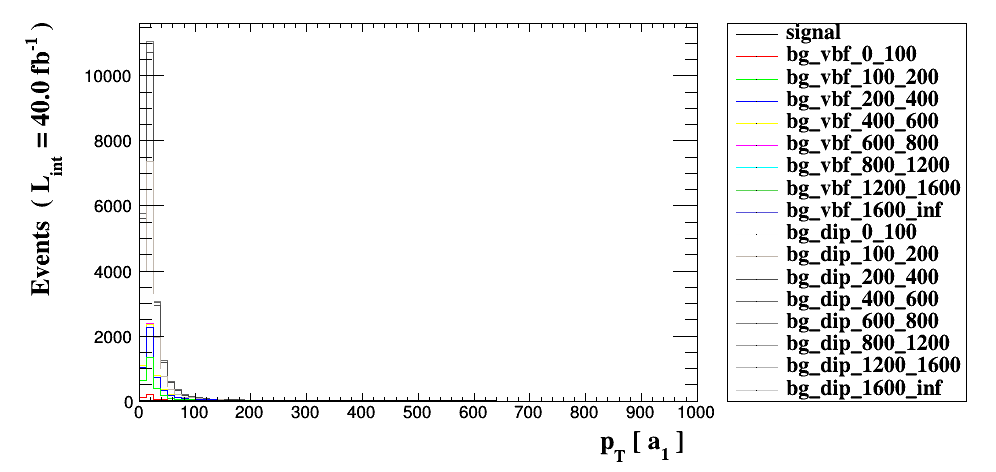
\includegraphics[scale=0.45]{selection_11.png}\\
\caption{   }
  \end{center}
\end{figure}
      \newpage
\subsection{ Histogram 13}

\textbf{* Plot: THT}\\
   \begin{table}[H]
  \begin{center}
    \begin{tabular}{|m{23.0mm}|m{23.0mm}|m{18.0mm}|m{19.0mm}|m{19.0mm}|m{19.0mm}|m{19.0mm}|}
      \hline
      {\cellcolor{yellow}         Dataset}& {\cellcolor{yellow}         Integral}& {\cellcolor{yellow}         Entries per event}& {\cellcolor{yellow}         Mean}& {\cellcolor{yellow}         RMS}& {\cellcolor{yellow}         \% underflow}& {\cellcolor{yellow}         \% overflow}\\
      \hline
      {\cellcolor{white}         signal}& {\cellcolor{white}         1071}& {\cellcolor{white}         1.0}& {\cellcolor{white}         454.304}& {\cellcolor{white}         276.1}& {\cellcolor{green}         0.0}& {\cellcolor{green}         0.06799}\\
      \hline
      {\cellcolor{white}         bg\_vbf\_0\_100}& {\cellcolor{white}         364}& {\cellcolor{white}         1.0}& {\cellcolor{white}         86.2365}& {\cellcolor{white}         9.446}& {\cellcolor{green}         0.0}& {\cellcolor{green}         0.0}\\
      \hline
      {\cellcolor{white}         bg\_vbf\_100\_200}& {\cellcolor{white}         2253}& {\cellcolor{white}         1.0}& {\cellcolor{white}         148.868}& {\cellcolor{white}         28.12}& {\cellcolor{green}         0.0}& {\cellcolor{green}         0.0}\\
      \hline
      {\cellcolor{white}         bg\_vbf\_200\_400}& {\cellcolor{white}         2038}& {\cellcolor{white}         1.0}& {\cellcolor{white}         269.397}& {\cellcolor{white}         51.71}& {\cellcolor{green}         0.0}& {\cellcolor{green}         0.0}\\
      \hline
      {\cellcolor{white}         bg\_vbf\_400\_600}& {\cellcolor{white}         279}& {\cellcolor{white}         1.0}& {\cellcolor{white}         470.153}& {\cellcolor{white}         53.21}& {\cellcolor{green}         0.0}& {\cellcolor{green}         0.0}\\
      \hline
      {\cellcolor{white}         bg\_vbf\_600\_800}& {\cellcolor{white}         47.9}& {\cellcolor{white}         1.0}& {\cellcolor{white}         673.649}& {\cellcolor{white}         54.12}& {\cellcolor{green}         0.0}& {\cellcolor{green}         0.0}\\
      \hline
      {\cellcolor{white}         bg\_vbf\_800\_1200}& {\cellcolor{white}         12.1}& {\cellcolor{white}         1.0}& {\cellcolor{white}         913.399}& {\cellcolor{white}         95.85}& {\cellcolor{green}         0.0}& {\cellcolor{green}         0.0}\\
      \hline
      {\cellcolor{white}         bg\_vbf\_1200\_1600}& {\cellcolor{white}         0.677}& {\cellcolor{white}         1.0}& {\cellcolor{white}         1317.14}& {\cellcolor{white}         96.31}& {\cellcolor{green}         0.0}& {\cellcolor{green}         0.0}\\
      \hline
      {\cellcolor{white}         bg\_vbf\_1600\_inf}& {\cellcolor{white}         0.0489}& {\cellcolor{white}         1.0}& {\cellcolor{white}         1746.14}& {\cellcolor{white}         153.9}& {\cellcolor{orange}         0.0}& {\cellcolor{orange}         6.375}\\
      \hline
      {\cellcolor{white}         bg\_dip\_0\_100}& {\cellcolor{white}         1767}& {\cellcolor{white}         1.0}& {\cellcolor{white}         85.9542}& {\cellcolor{white}         9.466}& {\cellcolor{green}         0.0}& {\cellcolor{green}         0.0}\\
      \hline
      {\cellcolor{white}         bg\_dip\_100\_200}& {\cellcolor{white}         8038}& {\cellcolor{white}         1.0}& {\cellcolor{white}         147.775}& {\cellcolor{white}         28.3}& {\cellcolor{green}         0.0}& {\cellcolor{green}         0.0}\\
      \hline
      {\cellcolor{white}         bg\_dip\_200\_400}& {\cellcolor{white}         6955}& {\cellcolor{white}         1.0}& {\cellcolor{white}         263.454}& {\cellcolor{white}         48.38}& {\cellcolor{green}         0.0}& {\cellcolor{green}         0.0}\\
      \hline
      {\cellcolor{white}         bg\_dip\_400\_600}& {\cellcolor{white}         638}& {\cellcolor{white}         1.0}& {\cellcolor{white}         467.106}& {\cellcolor{white}         52.56}& {\cellcolor{green}         0.0}& {\cellcolor{green}         0.0}\\
      \hline
      {\cellcolor{white}         bg\_dip\_600\_800}& {\cellcolor{white}         89.9}& {\cellcolor{white}         1.0}& {\cellcolor{white}         671.611}& {\cellcolor{white}         53.46}& {\cellcolor{green}         0.0}& {\cellcolor{green}         0.0}\\
      \hline
      {\cellcolor{white}         bg\_dip\_800\_1200}& {\cellcolor{white}         21.9}& {\cellcolor{white}         1.0}& {\cellcolor{white}         912.241}& {\cellcolor{white}         94.72}& {\cellcolor{green}         0.0}& {\cellcolor{green}         0.0}\\
      \hline
      {\cellcolor{white}         bg\_dip\_1200\_1600}& {\cellcolor{white}         1.31}& {\cellcolor{white}         1.0}& {\cellcolor{white}         1317.23}& {\cellcolor{white}         95.31}& {\cellcolor{green}         0.0}& {\cellcolor{green}         0.0}\\
      \hline
      {\cellcolor{white}         bg\_dip\_1600\_inf}& {\cellcolor{white}         0.0878}& {\cellcolor{white}         1.0}& {\cellcolor{white}         1749.76}& {\cellcolor{white}         155.9}& {\cellcolor{orange}         0.0}& {\cellcolor{orange}         8.029}\\
\hline
    \end{tabular}
  \end{center}
\end{table}

\begin{figure}[H]
  \begin{center}
    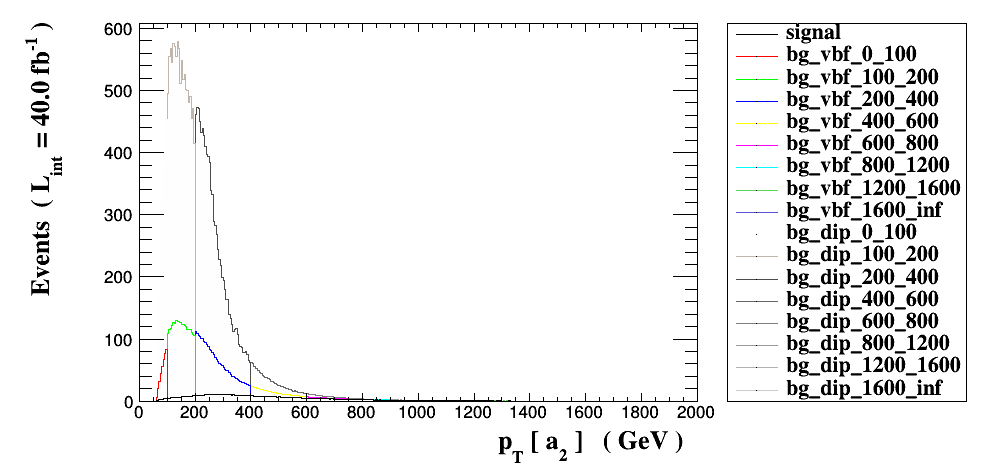
\includegraphics[scale=0.45]{selection_12.png}\\
\caption{   }
  \end{center}
\end{figure}
      \newpage
\subsection{ Histogram 14}

\textbf{* Plot: MET}\\
   \begin{table}[H]
  \begin{center}
    \begin{tabular}{|m{23.0mm}|m{23.0mm}|m{18.0mm}|m{19.0mm}|m{19.0mm}|m{19.0mm}|m{19.0mm}|}
      \hline
      {\cellcolor{yellow}         Dataset}& {\cellcolor{yellow}         Integral}& {\cellcolor{yellow}         Entries per event}& {\cellcolor{yellow}         Mean}& {\cellcolor{yellow}         RMS}& {\cellcolor{yellow}         \% underflow}& {\cellcolor{yellow}         \% overflow}\\
      \hline
      {\cellcolor{white}         signal}& {\cellcolor{white}         1071}& {\cellcolor{white}         1.0}& {\cellcolor{white}         7.65721e-09}& {\cellcolor{white}         9.954e-09}& {\cellcolor{green}         0.0}& {\cellcolor{green}         0.0}\\
      \hline
      {\cellcolor{white}         bg\_vbf\_0\_100}& {\cellcolor{white}         364}& {\cellcolor{white}         1.0}& {\cellcolor{white}         6.1357e-10}& {\cellcolor{white}         4.53e-10}& {\cellcolor{green}         0.0}& {\cellcolor{green}         0.0}\\
      \hline
      {\cellcolor{white}         bg\_vbf\_100\_200}& {\cellcolor{white}         2253}& {\cellcolor{white}         1.0}& {\cellcolor{white}         9.9577e-10}& {\cellcolor{white}         1.139e-09}& {\cellcolor{green}         0.0}& {\cellcolor{green}         0.0}\\
      \hline
      {\cellcolor{white}         bg\_vbf\_200\_400}& {\cellcolor{white}         2038}& {\cellcolor{white}         1.0}& {\cellcolor{white}         3.24261e-09}& {\cellcolor{white}         2.215e-09}& {\cellcolor{green}         0.0}& {\cellcolor{green}         0.0}\\
      \hline
      {\cellcolor{white}         bg\_vbf\_400\_600}& {\cellcolor{white}         279}& {\cellcolor{white}         1.0}& {\cellcolor{white}         4.57408e-09}& {\cellcolor{white}         2.638e-09}& {\cellcolor{green}         0.0}& {\cellcolor{green}         0.0}\\
      \hline
      {\cellcolor{white}         bg\_vbf\_600\_800}& {\cellcolor{white}         47.9}& {\cellcolor{white}         1.0}& {\cellcolor{white}         4.96938e-09}& {\cellcolor{white}         2.751e-09}& {\cellcolor{green}         0.0}& {\cellcolor{green}         0.0}\\
      \hline
      {\cellcolor{white}         bg\_vbf\_800\_1200}& {\cellcolor{white}         12.1}& {\cellcolor{white}         1.0}& {\cellcolor{white}         5.28099e-09}& {\cellcolor{white}         3.228e-09}& {\cellcolor{green}         0.0}& {\cellcolor{green}         0.0}\\
      \hline
      {\cellcolor{white}         bg\_vbf\_1200\_1600}& {\cellcolor{white}         0.677}& {\cellcolor{white}         1.0}& {\cellcolor{white}         7.45383e-09}& {\cellcolor{white}         9.4e-09}& {\cellcolor{green}         0.0}& {\cellcolor{green}         0.0}\\
      \hline
      {\cellcolor{white}         bg\_vbf\_1600\_inf}& {\cellcolor{white}         0.0489}& {\cellcolor{white}         1.0}& {\cellcolor{white}         1.20778e-08}& {\cellcolor{white}         1.632e-08}& {\cellcolor{green}         0.0}& {\cellcolor{green}         0.0}\\
      \hline
      {\cellcolor{white}         bg\_dip\_0\_100}& {\cellcolor{white}         1767}& {\cellcolor{white}         1.0}& {\cellcolor{white}         6.0389e-10}& {\cellcolor{white}         5.254e-10}& {\cellcolor{green}         0.0}& {\cellcolor{green}         0.0}\\
      \hline
      {\cellcolor{white}         bg\_dip\_100\_200}& {\cellcolor{white}         8038}& {\cellcolor{white}         1.0}& {\cellcolor{white}         1.04034e-09}& {\cellcolor{white}         1.192e-09}& {\cellcolor{green}         0.0}& {\cellcolor{green}         0.0}\\
      \hline
      {\cellcolor{white}         bg\_dip\_200\_400}& {\cellcolor{white}         6955}& {\cellcolor{white}         1.0}& {\cellcolor{white}         3.18901e-09}& {\cellcolor{white}         2.202e-09}& {\cellcolor{green}         0.0}& {\cellcolor{green}         0.0}\\
      \hline
      {\cellcolor{white}         bg\_dip\_400\_600}& {\cellcolor{white}         638}& {\cellcolor{white}         1.0}& {\cellcolor{white}         4.48357e-09}& {\cellcolor{white}         2.597e-09}& {\cellcolor{green}         0.0}& {\cellcolor{green}         0.0}\\
      \hline
      {\cellcolor{white}         bg\_dip\_600\_800}& {\cellcolor{white}         89.9}& {\cellcolor{white}         1.0}& {\cellcolor{white}         4.82999e-09}& {\cellcolor{white}         2.653e-09}& {\cellcolor{green}         0.0}& {\cellcolor{green}         0.0}\\
      \hline
      {\cellcolor{white}         bg\_dip\_800\_1200}& {\cellcolor{white}         21.9}& {\cellcolor{white}         1.0}& {\cellcolor{white}         5.14727e-09}& {\cellcolor{white}         3.708e-09}& {\cellcolor{green}         0.0}& {\cellcolor{green}         0.0}\\
      \hline
      {\cellcolor{white}         bg\_dip\_1200\_1600}& {\cellcolor{white}         1.31}& {\cellcolor{white}         1.0}& {\cellcolor{white}         7.65407e-09}& {\cellcolor{white}         1.043e-08}& {\cellcolor{green}         0.0}& {\cellcolor{green}         0.0}\\
      \hline
      {\cellcolor{white}         bg\_dip\_1600\_inf}& {\cellcolor{white}         0.0878}& {\cellcolor{white}         1.0}& {\cellcolor{white}         9.90329e-09}& {\cellcolor{white}         1.373e-08}& {\cellcolor{green}         0.0}& {\cellcolor{green}         0.0}\\
\hline
    \end{tabular}
  \end{center}
\end{table}

\begin{figure}[H]
  \begin{center}
    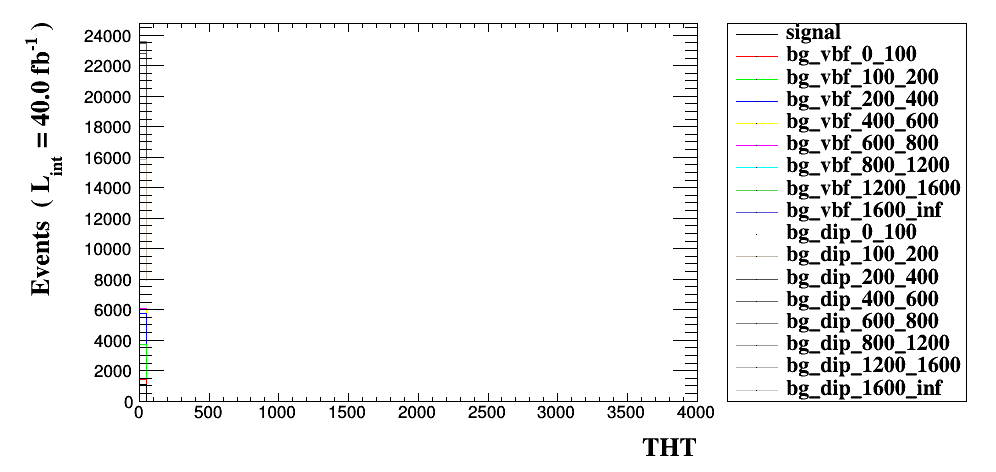
\includegraphics[scale=0.45]{selection_13.png}\\
\caption{   }
  \end{center}
\end{figure}
      \newpage
\subsection{ Histogram 15}

\textbf{* Plot: TET}\\
   \begin{table}[H]
  \begin{center}
    \begin{tabular}{|m{23.0mm}|m{23.0mm}|m{18.0mm}|m{19.0mm}|m{19.0mm}|m{19.0mm}|m{19.0mm}|}
      \hline
      {\cellcolor{yellow}         Dataset}& {\cellcolor{yellow}         Integral}& {\cellcolor{yellow}         Entries per event}& {\cellcolor{yellow}         Mean}& {\cellcolor{yellow}         RMS}& {\cellcolor{yellow}         \% underflow}& {\cellcolor{yellow}         \% overflow}\\
      \hline
      {\cellcolor{white}         signal}& {\cellcolor{white}         1071}& {\cellcolor{white}         1.0}& {\cellcolor{white}         1369.75}& {\cellcolor{white}         757.3}& {\cellcolor{red}         0.0}& {\cellcolor{red}         63.1}\\
      \hline
      {\cellcolor{white}         bg\_vbf\_0\_100}& {\cellcolor{white}         364}& {\cellcolor{white}         1.0}& {\cellcolor{white}         140.264}& {\cellcolor{white}         32.73}& {\cellcolor{green}         0.0}& {\cellcolor{green}         0.003329}\\
      \hline
      {\cellcolor{white}         bg\_vbf\_100\_200}& {\cellcolor{white}         2253}& {\cellcolor{white}         1.0}& {\cellcolor{white}         219.969}& {\cellcolor{white}         56.88}& {\cellcolor{green}         0.0}& {\cellcolor{green}         0.006239}\\
      \hline
      {\cellcolor{white}         bg\_vbf\_200\_400}& {\cellcolor{white}         2038}& {\cellcolor{white}         1.0}& {\cellcolor{white}         373.339}& {\cellcolor{white}         101.3}& {\cellcolor{green}         0.0}& {\cellcolor{green}         0.06772}\\
      \hline
      {\cellcolor{white}         bg\_vbf\_400\_600}& {\cellcolor{white}         279}& {\cellcolor{white}         1.0}& {\cellcolor{white}         628.497}& {\cellcolor{white}         147.8}& {\cellcolor{green}         0.0}& {\cellcolor{green}         2.599}\\
      \hline
      {\cellcolor{white}         bg\_vbf\_600\_800}& {\cellcolor{white}         47.9}& {\cellcolor{white}         1.0}& {\cellcolor{white}         876.628}& {\cellcolor{white}         197.5}& {\cellcolor{red}         0.0}& {\cellcolor{red}         21.09}\\
      \hline
      {\cellcolor{white}         bg\_vbf\_800\_1200}& {\cellcolor{white}         12.1}& {\cellcolor{white}         1.0}& {\cellcolor{white}         1161.77}& {\cellcolor{white}         278.1}& {\cellcolor{red}         0.0}& {\cellcolor{red}         66.2}\\
      \hline
      {\cellcolor{white}         bg\_vbf\_1200\_1600}& {\cellcolor{white}         0.677}& {\cellcolor{white}         1.0}& {\cellcolor{white}         1640.52}& {\cellcolor{white}         394.6}& {\cellcolor{red}         0.0}& {\cellcolor{red}         100.0}\\
      \hline
      {\cellcolor{white}         bg\_vbf\_1600\_inf}& {\cellcolor{white}         0.0489}& {\cellcolor{white}         1.0}& {\cellcolor{white}         2191.87}& {\cellcolor{white}         630.1}& {\cellcolor{red}         0.0}& {\cellcolor{red}         100.0}\\
      \hline
      {\cellcolor{white}         bg\_dip\_0\_100}& {\cellcolor{white}         1767}& {\cellcolor{white}         1.0}& {\cellcolor{white}         138.089}& {\cellcolor{white}         31.72}& {\cellcolor{green}         0.0}& {\cellcolor{green}         0.0}\\
      \hline
      {\cellcolor{white}         bg\_dip\_100\_200}& {\cellcolor{white}         8038}& {\cellcolor{white}         1.0}& {\cellcolor{white}         217.607}& {\cellcolor{white}         59.35}& {\cellcolor{green}         0.0}& {\cellcolor{green}         0.0}\\
      \hline
      {\cellcolor{white}         bg\_dip\_200\_400}& {\cellcolor{white}         6955}& {\cellcolor{white}         1.0}& {\cellcolor{white}         360.182}& {\cellcolor{white}         100.9}& {\cellcolor{green}         0.0}& {\cellcolor{green}         0.03972}\\
      \hline
      {\cellcolor{white}         bg\_dip\_400\_600}& {\cellcolor{white}         638}& {\cellcolor{white}         1.0}& {\cellcolor{white}         617.218}& {\cellcolor{white}         158.6}& {\cellcolor{green}         0.0}& {\cellcolor{green}         3.545}\\
      \hline
      {\cellcolor{white}         bg\_dip\_600\_800}& {\cellcolor{white}         89.9}& {\cellcolor{white}         1.0}& {\cellcolor{white}         859.029}& {\cellcolor{white}         211.9}& {\cellcolor{red}         0.0}& {\cellcolor{red}         17.75}\\
      \hline
      {\cellcolor{white}         bg\_dip\_800\_1200}& {\cellcolor{white}         21.9}& {\cellcolor{white}         1.0}& {\cellcolor{white}         1145.8}& {\cellcolor{white}         305.2}& {\cellcolor{red}         0.0}& {\cellcolor{red}         58.76}\\
      \hline
      {\cellcolor{white}         bg\_dip\_1200\_1600}& {\cellcolor{white}         1.31}& {\cellcolor{white}         1.0}& {\cellcolor{white}         1593.83}& {\cellcolor{white}         420.7}& {\cellcolor{red}         0.0}& {\cellcolor{red}         100.0}\\
      \hline
      {\cellcolor{white}         bg\_dip\_1600\_inf}& {\cellcolor{white}         0.0878}& {\cellcolor{white}         1.0}& {\cellcolor{white}         2097.54}& {\cellcolor{white}         619.6}& {\cellcolor{red}         0.0}& {\cellcolor{red}         100.0}\\
\hline
    \end{tabular}
  \end{center}
\end{table}

\begin{figure}[H]
  \begin{center}
    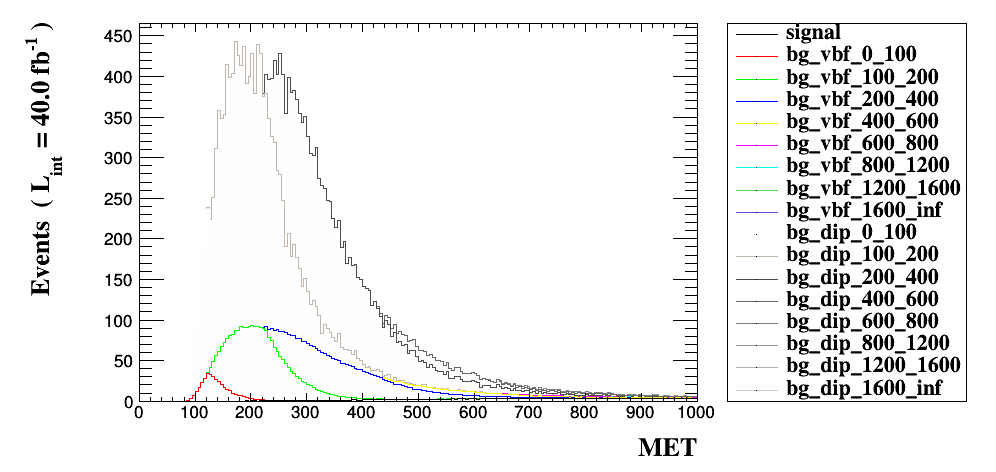
\includegraphics[scale=0.45]{selection_14.png}\\
\caption{   }
  \end{center}
\end{figure}
      \newpage
\subsection{ Histogram 16}

\textbf{* Plot: DELTAR ( a[1] , a[2] ) }\\
   \begin{table}[H]
  \begin{center}
    \begin{tabular}{|m{23.0mm}|m{23.0mm}|m{18.0mm}|m{19.0mm}|m{19.0mm}|m{19.0mm}|m{19.0mm}|}
      \hline
      {\cellcolor{yellow}         Dataset}& {\cellcolor{yellow}         Integral}& {\cellcolor{yellow}         Entries per event}& {\cellcolor{yellow}         Mean}& {\cellcolor{yellow}         RMS}& {\cellcolor{yellow}         \% underflow}& {\cellcolor{yellow}         \% overflow}\\
      \hline
      {\cellcolor{white}         signal}& {\cellcolor{white}         1071}& {\cellcolor{white}         1.0}& {\cellcolor{white}         2.73806}& {\cellcolor{white}         0.8532}& {\cellcolor{green}         0.0}& {\cellcolor{green}         0.0}\\
      \hline
      {\cellcolor{white}         bg\_vbf\_0\_100}& {\cellcolor{white}         364}& {\cellcolor{white}         1.0}& {\cellcolor{white}         2.63558}& {\cellcolor{white}         0.9837}& {\cellcolor{green}         0.0}& {\cellcolor{green}         0.0}\\
      \hline
      {\cellcolor{white}         bg\_vbf\_100\_200}& {\cellcolor{white}         2253}& {\cellcolor{white}         1.0}& {\cellcolor{white}         2.482}& {\cellcolor{white}         0.9847}& {\cellcolor{green}         0.0}& {\cellcolor{green}         0.0}\\
      \hline
      {\cellcolor{white}         bg\_vbf\_200\_400}& {\cellcolor{white}         2038}& {\cellcolor{white}         1.0}& {\cellcolor{white}         2.40629}& {\cellcolor{white}         0.9688}& {\cellcolor{green}         0.0}& {\cellcolor{green}         0.0}\\
      \hline
      {\cellcolor{white}         bg\_vbf\_400\_600}& {\cellcolor{white}         279}& {\cellcolor{white}         1.0}& {\cellcolor{white}         2.36998}& {\cellcolor{white}         0.9628}& {\cellcolor{green}         0.0}& {\cellcolor{green}         0.0}\\
      \hline
      {\cellcolor{white}         bg\_vbf\_600\_800}& {\cellcolor{white}         47.9}& {\cellcolor{white}         1.0}& {\cellcolor{white}         2.35535}& {\cellcolor{white}         0.9565}& {\cellcolor{green}         0.0}& {\cellcolor{green}         0.0}\\
      \hline
      {\cellcolor{white}         bg\_vbf\_800\_1200}& {\cellcolor{white}         12.1}& {\cellcolor{white}         1.0}& {\cellcolor{white}         2.34039}& {\cellcolor{white}         0.9474}& {\cellcolor{green}         0.0}& {\cellcolor{green}         0.0}\\
      \hline
      {\cellcolor{white}         bg\_vbf\_1200\_1600}& {\cellcolor{white}         0.677}& {\cellcolor{white}         1.0}& {\cellcolor{white}         2.33111}& {\cellcolor{white}         0.9391}& {\cellcolor{green}         0.0}& {\cellcolor{green}         0.0}\\
      \hline
      {\cellcolor{white}         bg\_vbf\_1600\_inf}& {\cellcolor{white}         0.0489}& {\cellcolor{white}         1.0}& {\cellcolor{white}         2.32373}& {\cellcolor{white}         0.9134}& {\cellcolor{green}         0.0}& {\cellcolor{green}         0.0}\\
      \hline
      {\cellcolor{white}         bg\_dip\_0\_100}& {\cellcolor{white}         1767}& {\cellcolor{white}         1.0}& {\cellcolor{white}         2.45807}& {\cellcolor{white}         0.911}& {\cellcolor{green}         0.0}& {\cellcolor{green}         0.0}\\
      \hline
      {\cellcolor{white}         bg\_dip\_100\_200}& {\cellcolor{white}         8038}& {\cellcolor{white}         1.0}& {\cellcolor{white}         2.30771}& {\cellcolor{white}         1.056}& {\cellcolor{green}         0.0}& {\cellcolor{green}         0.0}\\
      \hline
      {\cellcolor{white}         bg\_dip\_200\_400}& {\cellcolor{white}         6955}& {\cellcolor{white}         1.0}& {\cellcolor{white}         2.29185}& {\cellcolor{white}         1.123}& {\cellcolor{green}         0.0}& {\cellcolor{green}         0.0}\\
      \hline
      {\cellcolor{white}         bg\_dip\_400\_600}& {\cellcolor{white}         638}& {\cellcolor{white}         1.0}& {\cellcolor{white}         2.38449}& {\cellcolor{white}         1.211}& {\cellcolor{green}         0.0}& {\cellcolor{green}         0.0}\\
      \hline
      {\cellcolor{white}         bg\_dip\_600\_800}& {\cellcolor{white}         89.9}& {\cellcolor{white}         1.0}& {\cellcolor{white}         2.4517}& {\cellcolor{white}         1.258}& {\cellcolor{green}         0.0}& {\cellcolor{green}         0.0}\\
      \hline
      {\cellcolor{white}         bg\_dip\_800\_1200}& {\cellcolor{white}         21.9}& {\cellcolor{white}         1.0}& {\cellcolor{white}         2.51942}& {\cellcolor{white}         1.28}& {\cellcolor{green}         0.0}& {\cellcolor{green}         0.0}\\
      \hline
      {\cellcolor{white}         bg\_dip\_1200\_1600}& {\cellcolor{white}         1.31}& {\cellcolor{white}         1.0}& {\cellcolor{white}         2.59316}& {\cellcolor{white}         1.343}& {\cellcolor{green}         0.0}& {\cellcolor{green}         0.0}\\
      \hline
      {\cellcolor{white}         bg\_dip\_1600\_inf}& {\cellcolor{white}         0.0878}& {\cellcolor{white}         1.0}& {\cellcolor{white}         2.7138}& {\cellcolor{white}         1.335}& {\cellcolor{green}         0.0}& {\cellcolor{green}         0.0}\\
\hline
    \end{tabular}
  \end{center}
\end{table}

\begin{figure}[H]
  \begin{center}
    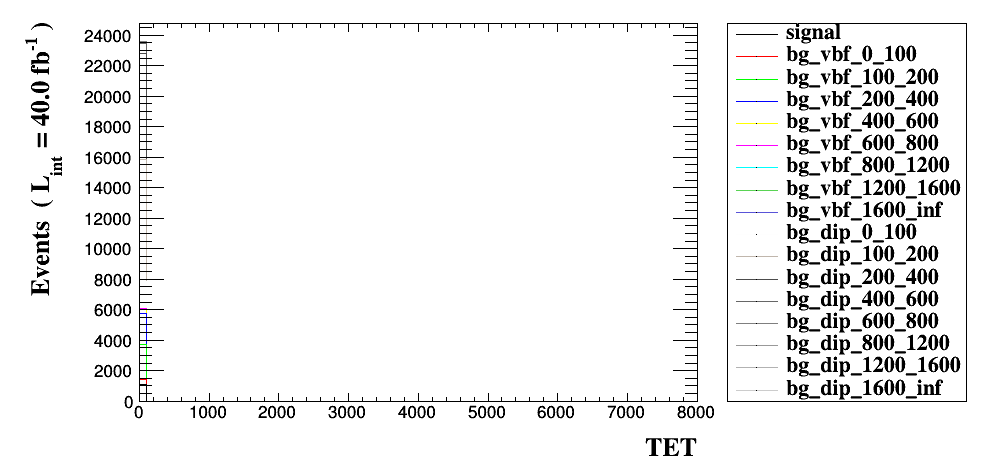
\includegraphics[scale=0.45]{selection_15.png}\\
\caption{   }
  \end{center}
\end{figure}
      \newpage
\subsection{ Histogram 17}

\textbf{* Plot: sdETA ( a[1] a[2] ) }\\
   \begin{table}[H]
  \begin{center}
    \begin{tabular}{|m{23.0mm}|m{23.0mm}|m{18.0mm}|m{19.0mm}|m{19.0mm}|m{19.0mm}|m{19.0mm}|}
      \hline
      {\cellcolor{yellow}         Dataset}& {\cellcolor{yellow}         Integral}& {\cellcolor{yellow}         Entries per event}& {\cellcolor{yellow}         Mean}& {\cellcolor{yellow}         RMS}& {\cellcolor{yellow}         \% underflow}& {\cellcolor{yellow}         \% overflow}\\
      \hline
      {\cellcolor{white}         signal}& {\cellcolor{white}         1071}& {\cellcolor{white}         1.0}& {\cellcolor{white}         0.00306436}& {\cellcolor{white}         1.57}& {\cellcolor{green}         0.001528}& {\cellcolor{green}         0.001528}\\
      \hline
      {\cellcolor{white}         bg\_vbf\_0\_100}& {\cellcolor{white}         364}& {\cellcolor{white}         1.0}& {\cellcolor{white}         0.011358}& {\cellcolor{white}         1.887}& {\cellcolor{green}         0.0}& {\cellcolor{green}         0.0}\\
      \hline
      {\cellcolor{white}         bg\_vbf\_100\_200}& {\cellcolor{white}         2253}& {\cellcolor{white}         1.0}& {\cellcolor{white}         0.00157671}& {\cellcolor{white}         1.85}& {\cellcolor{green}         0.0}& {\cellcolor{green}         0.0}\\
      \hline
      {\cellcolor{white}         bg\_vbf\_200\_400}& {\cellcolor{white}         2038}& {\cellcolor{white}         1.0}& {\cellcolor{white}         0.00581319}& {\cellcolor{white}         1.788}& {\cellcolor{green}         0.0}& {\cellcolor{green}         0.0}\\
      \hline
      {\cellcolor{white}         bg\_vbf\_400\_600}& {\cellcolor{white}         279}& {\cellcolor{white}         1.0}& {\cellcolor{white}         0.00688874}& {\cellcolor{white}         1.766}& {\cellcolor{green}         0.0}& {\cellcolor{green}         0.0}\\
      \hline
      {\cellcolor{white}         bg\_vbf\_600\_800}& {\cellcolor{white}         47.9}& {\cellcolor{white}         1.0}& {\cellcolor{white}         -0.0031434}& {\cellcolor{white}         1.757}& {\cellcolor{green}         0.0}& {\cellcolor{green}         0.0}\\
      \hline
      {\cellcolor{white}         bg\_vbf\_800\_1200}& {\cellcolor{white}         12.1}& {\cellcolor{white}         1.0}& {\cellcolor{white}         -0.0280331}& {\cellcolor{white}         1.742}& {\cellcolor{green}         0.0}& {\cellcolor{green}         0.0}\\
      \hline
      {\cellcolor{white}         bg\_vbf\_1200\_1600}& {\cellcolor{white}         0.677}& {\cellcolor{white}         1.0}& {\cellcolor{white}         0.0094622}& {\cellcolor{white}         1.738}& {\cellcolor{green}         0.0}& {\cellcolor{green}         0.0}\\
      \hline
      {\cellcolor{white}         bg\_vbf\_1600\_inf}& {\cellcolor{white}         0.0489}& {\cellcolor{white}         1.0}& {\cellcolor{white}         -0.0612251}& {\cellcolor{white}         1.68}& {\cellcolor{green}         0.0}& {\cellcolor{green}         0.0}\\
      \hline
      {\cellcolor{white}         bg\_dip\_0\_100}& {\cellcolor{white}         1767}& {\cellcolor{white}         1.0}& {\cellcolor{white}         -0.0927995}& {\cellcolor{white}         1.373}& {\cellcolor{green}         0.0}& {\cellcolor{green}         0.0}\\
      \hline
      {\cellcolor{white}         bg\_dip\_100\_200}& {\cellcolor{white}         8038}& {\cellcolor{white}         1.0}& {\cellcolor{white}         0.00715226}& {\cellcolor{white}         1.571}& {\cellcolor{green}         0.0}& {\cellcolor{green}         0.0}\\
      \hline
      {\cellcolor{white}         bg\_dip\_200\_400}& {\cellcolor{white}         6955}& {\cellcolor{white}         1.0}& {\cellcolor{white}         0.0184645}& {\cellcolor{white}         1.698}& {\cellcolor{green}         0.0}& {\cellcolor{green}         0.0}\\
      \hline
      {\cellcolor{white}         bg\_dip\_400\_600}& {\cellcolor{white}         638}& {\cellcolor{white}         1.0}& {\cellcolor{white}         -0.00432736}& {\cellcolor{white}         1.892}& {\cellcolor{green}         0.0}& {\cellcolor{green}         0.0}\\
      \hline
      {\cellcolor{white}         bg\_dip\_600\_800}& {\cellcolor{white}         89.9}& {\cellcolor{white}         1.0}& {\cellcolor{white}         0.0214844}& {\cellcolor{white}         2.018}& {\cellcolor{green}         0.0}& {\cellcolor{green}         0.0}\\
      \hline
      {\cellcolor{white}         bg\_dip\_800\_1200}& {\cellcolor{white}         21.9}& {\cellcolor{white}         1.0}& {\cellcolor{white}         0.0326318}& {\cellcolor{white}         2.106}& {\cellcolor{green}         0.0}& {\cellcolor{green}         0.0}\\
      \hline
      {\cellcolor{white}         bg\_dip\_1200\_1600}& {\cellcolor{white}         1.31}& {\cellcolor{white}         1.0}& {\cellcolor{white}         0.0239735}& {\cellcolor{white}         2.232}& {\cellcolor{green}         0.0}& {\cellcolor{green}         0.0}\\
      \hline
      {\cellcolor{white}         bg\_dip\_1600\_inf}& {\cellcolor{white}         0.0878}& {\cellcolor{white}         1.0}& {\cellcolor{white}         -0.0233956}& {\cellcolor{white}         2.409}& {\cellcolor{green}         0.0}& {\cellcolor{green}         0.0}\\
\hline
    \end{tabular}
  \end{center}
\end{table}

\begin{figure}[H]
  \begin{center}
    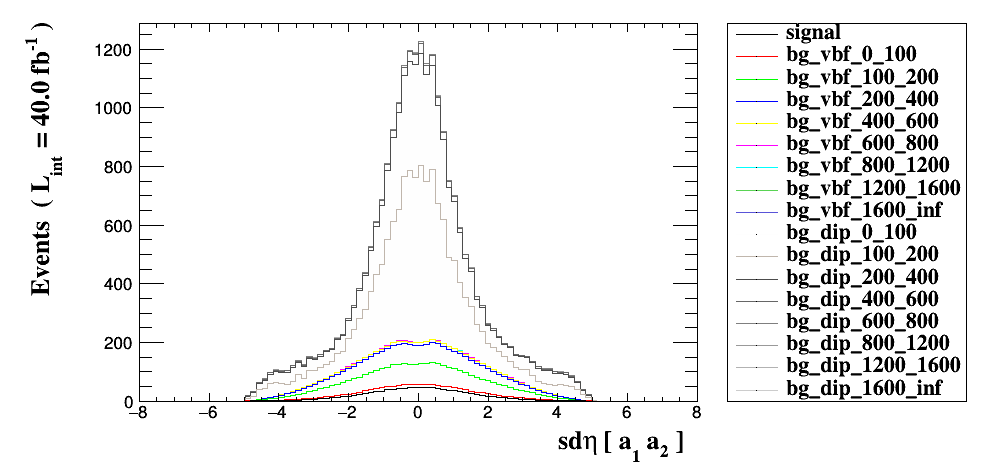
\includegraphics[scale=0.45]{selection_16.png}\\
\caption{   }
  \end{center}
\end{figure}
      % -----------------------------------------------------------------------------
%                                SECTION Summary                                
% -----------------------------------------------------------------------------
\newpage
\section{ Summary}

\subsection{Cut-flow charts}

\begin{itemize}
  \item How to compare signal (S) and background (B): \textcolor{blue}{S/\-sqrt(S+B+(xB)**2)} .
   \item Object definition selections are indicated in cyan.  \item Reject and select are indicated by 'REJ' and 'SEL' respectively
\end{itemize}
\begin{table}[H]
  \begin{center}
    \begin{tabular}{|m{36.0mm}|m{36.0mm}|m{36.0mm}|m{33.0mm}|}
      \hline
      {\cellcolor{yellow}        Cuts}& {\cellcolor{yellow}         Signal (S)}& {\cellcolor{yellow}         Background (B)}& {\cellcolor{yellow}         S vs B}\\
      \hline
      {\cellcolor{white}         Initial (no cut)}& {\cellcolor{white}         4094.08 +/\-- 1.13}& {\cellcolor{white}         4113516 +/\-- 4877}& {\cellcolor{white}         2.01760 +/\-- 0.00132}\\
      \hline
      {\cellcolor{white} SEL: 30.0 > PT > 30.0}& {\cellcolor{white}         3815.6 +/\-- 16.1}& {\cellcolor{white}         2130189 +/\-- 2200}& {\cellcolor{white}         2.6119 +/\-- 0.0111}\\
      \hline
      {\cellcolor{white} SEL: sdETA ( jets[1] jets[2] ) > 3.6 or sdETA ( je}& {\cellcolor{white}         1214.2 +/\-- 29.2}& {\cellcolor{white}         133999 +/\-- 378}& {\cellcolor{white}         3.3021 +/\-- 0.0793}\\
      \hline
      {\cellcolor{white} SEL: M ( jets[1] jets[2] ) > 750.0}& {\cellcolor{white}         1071.9 +/\-- 28.1}& {\cellcolor{white}         22509 +/\-- 145}& {\cellcolor{white}         6.98 +/\-- 0.18}\\
\hline
    \end{tabular}
  \end{center}
\end{table}

\end{document}
